%%%%%%%%%%%%%%%%%%%%%%%%%%%%%%%%%%%%%%%%%%%%%%%%%%%
%% LaTeX book template                           %%
%% Author:  Amber Jain (http://amberj.devio.us/) %%
%% License: ISC license                          %%
%%%%%%%%%%%%%%%%%%%%%%%%%%%%%%%%%%%%%%%%%%%%%%%%%%%

\documentclass[a4paper,11pt]{book}
\usepackage[T1]{fontenc}
\usepackage[utf8]{inputenc}
\usepackage{lmodern}
%%%%%%%%%%%%%%%%%%%%%%%%%%%%%%%%%%%%%%%%%%%%%%%%%%%%%%%%%
% Source: http://en.wikibooks.org/wiki/LaTeX/Hyperlinks %
%%%%%%%%%%%%%%%%%%%%%%%%%%%%%%%%%%%%%%%%%%%%%%%%%%%%%%%%%
\usepackage{hyperref}
\usepackage{graphicx}
\usepackage{float}
\usepackage{wrapfig}
\usepackage[english]{babel}
\usepackage{longtable}
\usepackage{listings}
\usepackage{color}
\usepackage{amsmath}
\usepackage{mathtools}
\lstset{frame=tb,
  language=VHDL,
  aboveskip=3mm,
  belowskip=3mm,
  showstringspaces=false,
  columns=flexible,
  basicstyle={\small\ttfamily},
  numbers=none,
  numberstyle=\tiny\color{gray},
  keywordstyle=\color{blue},
  commentstyle=\color{dkgreen},
  stringstyle=\color{mauve},
  breaklines=true,
  breakatwhitespace=true,
  tabsize=3
}

%%%%%%%%%%%%%%%%%%%%%%%%%%%%%%%%%%%%%%%%%%%%%%%%%%%%%%%%%%%%%%%%%%%%%%%%%%%%%%%%
% 'dedication' environment: To add a dedication paragraph at the start of book %
% Source: http://www.tug.org/pipermail/texhax/2010-June/015184.html            %
%%%%%%%%%%%%%%%%%%%%%%%%%%%%%%%%%%%%%%%%%%%%%%%%%%%%%%%%%%%%%%%%%%%%%%%%%%%%%%%%
\newenvironment{dedication}
{
   \cleardoublepage
   \thispagestyle{empty}
   \vspace*{\stretch{1}}
   \hfill\begin{minipage}[t]{0.66\textwidth}
   \raggedright
}
{
   \end{minipage}
   \vspace*{\stretch{3}}
   \clearpage
}

%%%%%%%%%%%%%%%%%%%%%%%%%%%%%%%%%%%%%%%%%%%%%%%%
% Chapter quote at the start of chapter        %
% Source: http://tex.stackexchange.com/a/53380 %
%%%%%%%%%%%%%%%%%%%%%%%%%%%%%%%%%%%%%%%%%%%%%%%%
\makeatletter
\renewcommand{\@chapapp}{}% Not necessary...
\newenvironment{chapquote}[2][2em]
  {\setlength{\@tempdima}{#1}%
   \def\chapquote@author{#2}%
   \parshape 1 \@tempdima \dimexpr\textwidth-2\@tempdima\relax%
   \itshape}
  {\par\normalfont\hfill--\ \chapquote@author\hspace*{\@tempdima}\par\bigskip}
\makeatother

\definecolor{dkgreen}{rgb}{0,0.6,0}
\definecolor{gray}{rgb}{0.5,0.5,0.5}
\definecolor{mauve}{rgb}{0.58,0,0.82}

%%%%%%%%%%%%%%%%%%%%%%%%%%%%%%%%%%%%%%%%%%%%%%%%%%%
% First page of book which contains 'stuff' like: %
%  - Book title, subtitle                         %
%  - Book author name                             %
%%%%%%%%%%%%%%%%%%%%%%%%%%%%%%%%%%%%%%%%%%%%%%%%%%%

% Book's title and subtitle
\title{\Huge \textbf{Digital Lab Notebook} \\ \LARGE ECE 3450-001 Digital Electronics \\ \Large Villanova University \\ Dr. Jupina}
% Author
\author{\Large \textsc{Brian Sakhuja}}


\begin{document}

\frontmatter
\maketitle

%%%%%%%%%%%%%%%%%%%%%%%%%%%%%%%%%%%%%%%%%%%%%%%%%%%%%%%%%%%%%%%
% Add a dedication paragraph to dedicate your book to someone %
%%%%%%%%%%%%%%%%%%%%%%%%%%%%%%%%%%%%%%%%%%%%%%%%%%%%%%%%%%%%%%%
\begin{dedication}
Dedicated to Dr. Caverly's moustache.
\end{dedication}

%%%%%%%%%%%%%%%%%%%%%%%%%%%%%%%%%%%%%%%%%%%%%%%%%%%%%%%%%%%%%%%%%%%%%%%%
% Auto-generated table of contents, list of figures and list of tables %
%%%%%%%%%%%%%%%%%%%%%%%%%%%%%%%%%%%%%%%%%%%%%%%%%%%%%%%%%%%%%%%%%%%%%%%%
\tableofcontents
\listoffigures
\listoftables

\mainmatter


%%%%%%%%%%%%%%%%
% PRACTICUM 1 %
%%%%%%%%%%%%%%%%
\chapter{Practicum 1: Properties of Digital Circuits}
\section{Part 1: Voltage Transfer Characteristics}
\subsection{Overview}
In this part of the practicum, we observe properties of a low-power Shottky Transistor-Transistor Logic (LS-TTL) gate and Complementary Metal-Oxide Semiconductor (CMOS) gate.  We used data sheets for both the 74LS04 and CMOS 4069 devices along with oscilloscope readings and manual calculations to evaluate the characteristics of these two different technologies.  Using these characteristics, we can determine the advantages and disadvantages of each gate technology.
\subsection{Purpose}
The purpose of this part of the practicum is to observe the input/output characteristics of a LS-TTL inverter (74LS04) and a CMOS Hex inverter (CMOS 4069).  We can determine the thresholds for a logic "low" and logic "high" state for these devices by examining their output responses on an oscilloscope. Ideally, we would like an inverter to have two discrete states: low or high, where there is an infinite slope between the two states.  However, in reality, we will observe that there is some finite slope.
\subsection{Procedure}
A 0 to 5V sawtooth signal at 1kHz was set up using a function generator.  The sawtooth waveform was selected, frequency was set to 1kHz, and amplitude was set at $2.5V_{pp}$ to obtain a 5V amplitude.  Next, the offset of the waveform was set to $+1.25V$ to raise the signal by 2.5V.  The signal at this point is a 0 to 5V sawtooth at oscillating at 1kHz.  Using an oscilloscope, we checked that the signal is correct. Next, we set a power supply to give 5V.  Now, we build the circuit shown in Figure 1.5 using the 74LS04 chip. Using red wires for 5V power and black for 0V (ground), we wire up the circuit and turn the power supply and function generator on.  Using the oscilloscope, we then capture the output voltage as well as the input sawtooth signal.

Next, we capture the inverter gate's voltage transfer characteristic (VTC).  We press the \textbf{Horiz} button on the oscilloscope and then press \textbf{Time Mode} in the horizontal menu and hit \textbf{XY}. Using the vertical position and scaling knobs, we adjust the channel's position and scaling.  This display was captured and imported into Microsoft Word.  We add two lines with slope = -1 to determine the values of ${V_{IL}}$, ${V_{OH}}$, ${V_{IH}}$, and ${V_{OL}}$.  To obtain these values, place the lines on the XY plot where its slope is -1.  Then, we draw vertical lines down to the x-axis and horizontal lines to the y-axis.  Using the x and y division values in the top left of the oscilloscope display, we determine ${V_{IL}}$, ${V_{OH}}$, ${V_{IH}}$, and ${V_{OL}}$. ${V_{IL}}$ is located along the x-axis and is closest to the y-axis.  That is, ${V_{IL}}$ is smaller in value compared to ${V_{IH}}$.  ${V_{OL}}$ is located along the y-axis and is smaller in magnitude compared to ${V_{OH}}$.  ${V_{IL}}$ corresponds to ${V_{OH}}$ and ${V_{IH}}$ corresponds to ${V_{OL}}$.  These values were recorded and we repeat the procedure for the CMOS 4069 Hex inverter.
\subsection{Calculations, Data, and Graphs}
%Equations
Noise margin equations:
\begin{equation}
    NM_{H} = V_{OH} - V_{IH}
\end{equation}
\begin{equation}
    NM_{L} = V_{IL} - V_{OL}
\end{equation}
\begin{equation}
    NM = min(NM_{H}, NM_{L})
\end{equation}
%74LS04 prelab i chart
\begin{table}[ht]
\caption{74LS04} % title of Table
\centering % used for centering table
\begin{tabular}{|c|c|c|c|c|c|}
% centered columns (4 columns)
\hline %inserts double horizontal lines
Parameter & Min & Typical & Max & Measured & Units \\ [0.5ex]
% inserts table
%heading
\hline % inserts single horizontal line
Low level voltage input ${V_{IL}}$  & - & - & 0.8 & 0.7 & V \\
High level voltage input ${V_{IH}}$ & 2 & - & - & 1.0 & V \\
Low level voltage output ${V_{OL}}$ & - & 0.35 & 0.5 & 0.2 & V  \\
High level voltage output ${V_{OH}}$ & 2.7 & 3.4 & - & 4.3 & V  \\
Hence calculated noise margin & 0.3 & - & - & 0.5 & V  \\ [1ex] % [1ex] adds vertical space
\hline %inserts single line
\end{tabular}
\label{table:nonlin} % is used to refer this table in the text
\end{table}

%noise margin calculation for TTL
Noise margin calculation for 74LS04
  $$ NM_{H} = 4.3 - 1 = 3.3V $$
  $$ NM_{L} = 0.7 - 0.2 = 0.5V $$
  $$ NM = min(NM_{L}, NM_{H}) = 0.5V $$
   

%CMOS 4069 prelab i chart
\begin{table}[ht]
\caption{CMOS 4069} % title of Table
\centering % used for centering table
\begin{tabular}{|c|c|c|c|c|c|}
% centered columns (4 columns)
\hline %inserts double horizontal lines
Parameter & Min & Typical & Max & Measured & Units \\ [0.5ex]
% inserts table
%heading
\hline % inserts single horizontal line
Low level voltage input ${V_{IL}}$  & - & - & 2.5 & 2.6 & V \\
High level voltage input ${V_{IH}}$ & 4 & - & - & 2.9 & V \\
Low level voltage output ${V_{OL}}$ & - & - & 0.05 & 0.4 & V  \\
High level voltage output ${V_{OH}}$ & 4.95 & - & - & 4.5 & V  \\
Hence calculated noise margin & 0.95 & - & - & 1.6 & V  \\ [1ex] % [1ex] adds vertical space
\hline %inserts single line
\end{tabular}
\label{table:nonlin} % is used to refer this table in the text
\end{table}

%noise margin calculation for CMOS
Noise margin calculation for CMOS 4069
  $$ NM_{H} = 4.5 - 2.9 = 1.6V $$
  $$ NM_{L} = 2.6 - 0.4 = 2.2V $$
  $$ NM = min(NM_{L}, NM_{H}) = 1.6V $$

%oscilloscope displays
\begin{figure}
    \centering
    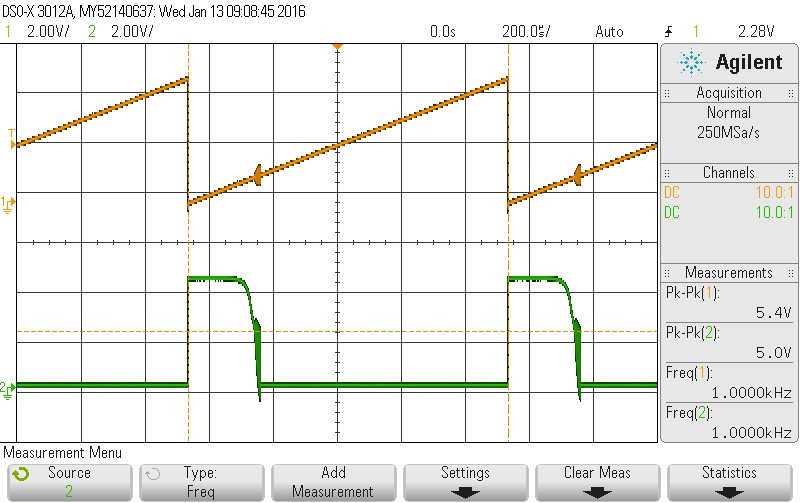
\includegraphics[width=\linewidth]{Practicum_1_Content/Part_i/TTL-input-output.jpg}
    \caption{TTL Input/Output}
\end{figure}
\begin{figure}
    \centering
    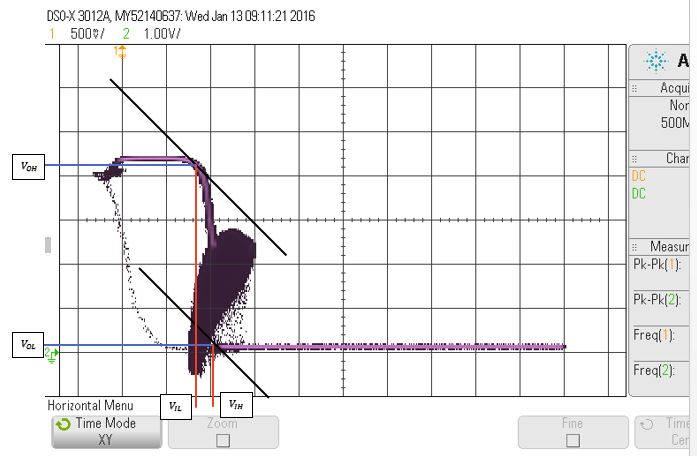
\includegraphics[width=\linewidth]{Practicum_1_Content/Part_i/TTL-xy.JPG}
    \caption{TTL XY}
\end{figure}
\begin{figure}
    \centering
    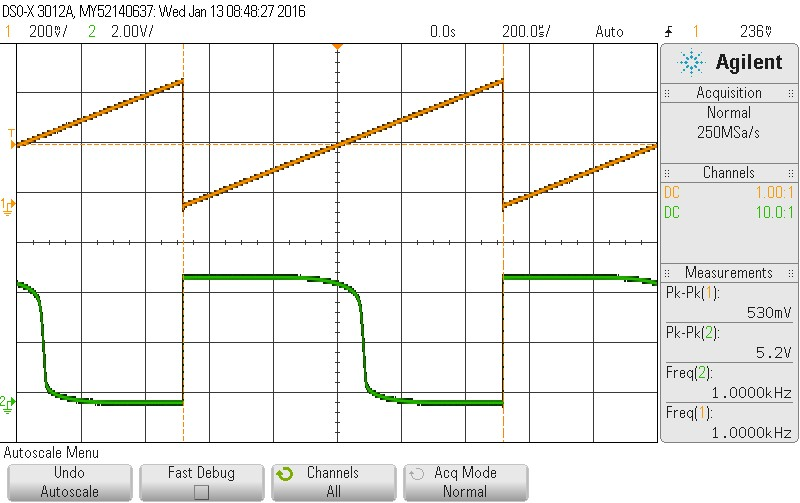
\includegraphics[width=\linewidth]{Practicum_1_Content/Part_i/cmos-input-output.jpg}
    \caption{CMOS Input/Output}
\end{figure}
\begin{figure}
    \centering
    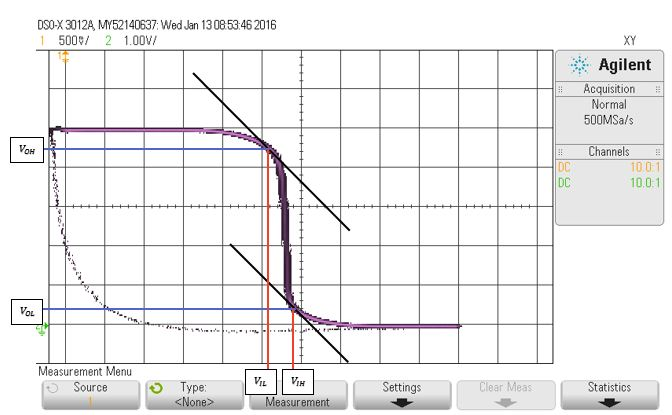
\includegraphics[width=\linewidth]{Practicum_1_Content/Part_i/cmos-xy.JPG}
    \caption{CMOS XY}
\end{figure}
\subsection{Discussion of Results}
For both the 74LS04 and CMOS 4069 technologies we observe the output is what we would expect from an inverter.  At low input voltages, we have a logic state 'high' and at high input voltages we observe a 'low' logic state output.

Referring to tables 1.1 and 1.2, we can see that some values come close to the expected, however, some do not.  Let us begin by discussing the 74LS04 device in table 1.1.  Our measured ${V_{IL}}$, ${V_{IH}}$, ${V_{OL}}$, and noise margin come fairly close to the expected values. Relatively, ${V_{OH}}$ had the largest discrepancy.

Looking at table 1.2 we now comment on the CMOS 4069 values. ${V_{IL}}$ and ${V_{OH}}$ come fairly close to the expected values.  However, ${V_{OL}}$ ${V_{IH}}$, and hence the calculated noise margin do not come as close as the other values do.
\subsection{Conclusions}
Errors could have arisen from the fact that the method of obtaining the voltage levels was not very precise.  Regardless, the general behavior of these technologies is what we expect.  We have observed their logic "low" and "high" output states using an oscilloscope.  Hence, we have determined the noise margins.  Comparing the 74LS04 and CMOS 4069, we can say that the CMOS performs much better.  The LS-TTL device had significantly higher levels of noise, while the CMOS had close to none.  Since the amount of noise was smaller, the CMOS device was easier to determine the input/output voltage highs and lows and hence the noise margin.
\subsection{Prelab}
See tables for the values obtained during prelab.
\begin{figure}
 \centering
    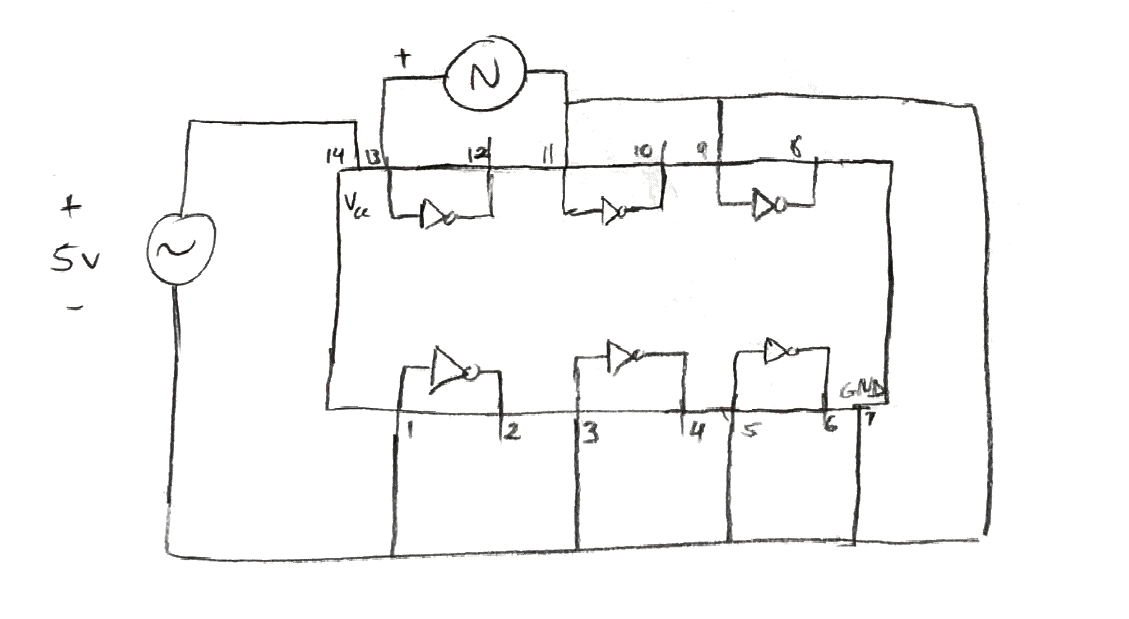
\includegraphics[width=\linewidth]{Practicum_1_Content/prelabCircuit.png}
    \caption{Pin Layout}
\end{figure}

%% Part 2 %%
\section{Part 2: Power Supply Current and Power Dissipation}
\subsection{Overview}
To further examine the characteristics of both the Low-power Schottky Transistor-Transistor Logic (74LS04) and Complementary Metal-Oxide Semiconductor (4069 CMOS hex inverter) devices, we examine the power supply current and power dissipation characteristics and compare and contrast their advantages and drawbacks.
\subsection{Purpose}
The purpose of this part of the practicum is to observe the power supply current and power dissipation behavior of both the 74LS04 and CMOS 4069 hex inverter as we increase the frequency.  These characteristics are critical when examining the performance of gate technologies and determining their suited applications.
\subsection{Procedure}
Using the same circuit setup as in Part 1 of this practicum, we wire up a multimeter in series with the 5V power supply such that the power supply's 5V terminal current flows through the meter to $V_{CC}$ of the LS7404 device.  The DC/quiescent supply current was measured by tying all inputs to low and recording the supply current.  Next, we tie all inputs to high and record the supply current.  We then compute the average supply current and then the average supply current per gate.  These values are shown in Table 1.3.

The subsequent steps are performed to measure the average supply current when the input is switching as a $50\%$ duty cycle square wave and when the output has a capacitive load. A 47 pF capacitor was added in between the gate output of each inverter and ground.  then all inputs were tied together and a 0-5V square wave was added to this common input (the same signal in Part I).  We then record the power supply current at frequencies of 1kHz, 10kHz, 100kHz, and 1MHz.  The average current and power dissipation per gate were computed and recorded in Table 1.4.

We repeat the procedure with the CMOS 4096 hex inverter.

Then we plot the power dissipated per gate versus frequency for each chip.  This is shown in Figure 1.6.
\subsection{Calculations, Data, and Graphs}
Equations
\begin{equation}
P_{AVG} = (\frac{I_{CC}}{6})(V_{CC})
\end{equation}
\begin{equation}
P_{AVG} = (\frac{I_{DD}}{6})(V_{DD})
\end{equation}
%74LS04 prelab ii charts
\begin{table}[ht]
\scriptsize
\caption{74LS04} % title of Table
\centering % used for centering table
\begin{tabular}{|c|c|c|c|c|}
\hline %inserts double horizontal lines
Parameter & Typical & Max & Measured & Units\\ [0.5ex]
% inserts table
%heading
\hline % inserts single horizontal line
Quiescent IC Supply Current, outputs high, ${I_{CCH}}$  & 1.2 & 2.4 & 1.240 & mA \\
Quiescent IC Supply Current, outputs low, ${I_{CCL}}$  & 3.6 & 6.6 & 3.865 & mA \\
Average quiescent IC supply current, ${I_{CC}}$  & 2.4 & 4.5 & 2.553 & mA \\
Average quiescent supply current per gate, ${I_{CC}/6}$  & 0.4 & 0.75 & 0.4254 & mA \\
Average quiescent power dissipation per gate  & 2.0 & 3.75 & 2.127 & mW \\ [1ex] % [1ex] adds vertical space
\hline %inserts single line
\end{tabular}
\label{table:nonlin} % is used to refer this table in the text
\end{table}
\begin{table}[ht]
\scriptsize
\caption{74LS04: Supply currents when switching at diff. frequencies with a 47pF capacitive load} % title of Table
\centering % used for centering table
\begin{tabular}{|c|c|c|c|c|c|}
\hline %inserts double horizontal lines
Parameter & 1kHz & 10kHz & 100kHz & 1MHz & Units\\ [0.5ex]
% inserts table
%heading
\hline % inserts single horizontal line
Average IC supply current, ${I_{CC}}$  & 2.545 & 2.563 & 2.728 & 4.380 & mA \\
Average supply current per gate, ${I_{CC}/6}$  & 0.4242 & 0.4272 & 0.4547 & 0.73 & mA \\
Average power dissipation per gate  & 2.121 & 2.274 & 2.273 & 3.65 & mW \\
Estimated power dissipation per gate (pre-lab)  & 2.4 & 2.45 & 2.5 & 3.75 & mW \\ [1ex] % [1ex] adds vertical space
\hline %inserts single line
\end{tabular}
\label{table:nonlin} % is used to refer this table in the text
\end{table}

%CMOS 4069 prelab ii charts
\begin{table}[ht]
\scriptsize
\caption{CMOS 4069 Hex Inverter} % title of Table
\centering % used for centering table
\begin{tabular}{|c|c|c|c|c|}
\hline %inserts double horizontal lines
Parameter & Typical & Max & Measured & Units\\ [0.5ex]
% inserts table
%heading
\hline % inserts single horizontal line
Quiescent IC Supply Current, outputs high, ${I_{DDH}}$  & - & - & 0 & mA \\
Quiescent IC Supply Current, outputs low, ${I_{DDL}}$  & - & - & 0 & mA \\
Average quiescent IC supply current, ${I_{DD}}$  & 0.0005 & 0.25 & 0 & mA \\
Average quiescent supply current per gate, ${I_{DD}/6}$  & ${8.33\times10^{-5}}$ & 0.0417 & 0 & mA \\
Average quiescent power dissipation per gate  & ${4.17\times10^{-4}}$ & 0.2085 & 0 & mW \\ [1ex] % [1ex] adds vertical space
\hline %inserts single line
\end{tabular}
\label{table:nonlin} % is used to refer this table in the text
\end{table}
\begin{table}[ht]
\scriptsize
\caption{CMOS 4069: Supply currents when switching at different frequencies with a 47pF capacitive load} % title of Table
\centering % used for centering table
\begin{tabular}{|c|c|c|c|c|c|}
\hline %inserts double horizontal lines
Parameter & 1kHz & 10kHz & 100kHz & 1MHz & Units\\ [0.5ex]
% inserts table
%heading
\hline % inserts single horizontal line
Average IC supply current, ${I_{CC}}$  & 1.9 & 18.7 & 186.6 & 1824 & uA \\
Average supply current per gate, ${I_{CC}/6}$  & 0.3167 & 3.117 & 31.1 & 304 & uA \\
Average power dissipation per gate  & 1.584 & 15.59 & 155.5 & 1520 & uW \\
Estimated power dissipation per gate (pre-lab)  & 0 & 25 & 250 & 2500 & mW \\ [1ex] % [1ex] adds vertical space
\hline %inserts single line
\end{tabular}
\label{table:nonlin} % is used to refer this table in the text
\end{table}

\begin{figure}
    \centering
    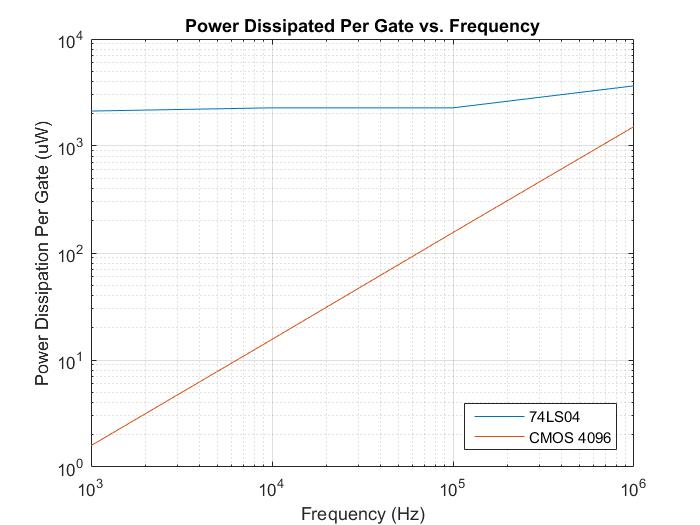
\includegraphics[width=\linewidth]{Practicum_1_Content/Part_ii/logGraph.jpg}
    \caption{Logarithmic Plot of Power Dissipaion Per Gate for Both Devices}
\end{figure}
\subsection{Discussion of Results}
We observe that our prelab calculated values for both devices closely match our values that we calculated from our measurements.  Specifically for the 74LS04 device in Table 1.3, our quiescent IC supply current values were very similar for both high and low outputs (1.2 vs 1.240 mA and 3.6 vs. 3.865 mA).  Therefore our average quiescent IC supply current was very similar (2.4 vs. 2.553 mA) as well as our average quiescent supply current per gate and average quiescent power dissipation per gate (0.4 vs 0.4254 mA and 2.0 vs. 2.127 mW).

For the CMOS 4069 hex inverter, we measured no quiescent IC supply current when outputs were either low or high.  The average quiescent power dissipation per gate was thus calculated to be 0 as well as shown in Table 1.5.

When we add a capacitive load of 47pF and switch our square wave input at different frequencies, the 74LS04 remained at a relatively constant power dissipation per gate when we increased the frequency.  However, the CMOS 4096 hex inverter increased power dissipation per gate when we increased the frequency as shown in Figure 1.6.
\subsection{Conclusions}
Looking at Figure 1.6, we can determine that depending on the application (one frequency versus another), one device might be preferable over another.  For example, if we have a low frequency application, the CMOS 4096 would be the choice device as it dissipates less power than the 74LS04 chip.  In the end, our prelab values mirror our measured results and we can observe the various drawbacks and advantages of each chip in terms of power dissipation and frequency.
\subsection{Prelab}
\begin{figure}
    \centering
    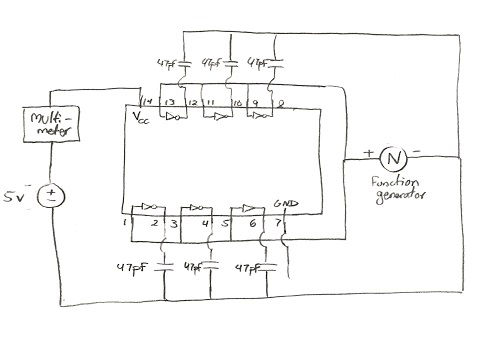
\includegraphics[width=\linewidth]{Practicum_1_Content/Part_ii/prelab.jpg}
    \caption{Prelab Circuit Diagram}
\end{figure}

See tables for prelab values.


% Part 3
\section{Part 3: Average Propagation Delay Time and Power-Delay Product}
\subsection{Overview}
In the third and final part of the practicum, we observe the average propagation delay time and power-delay product of both devices.
\subsection{Purpose}
Constructing a ring oscillator for the 74LS04 and CMOS 4096 allows us to easily measure the average propagation delay time and period of oscillation.  Thus, by obtaining these values, we can calculate the power delay product (PDP), an important property for any gate.
\subsection{Procedure}
We construct the circuit shown in Figure 1.10 using the 74LS04 device.  Each capacitor has a value of 47pF.  The period of the ring oscillator was measured and recorded using an oscilloscope.  A screen capture was taken of the oscilloscope display and is shown in Figure 1.8.  Then, Table 1.7 was completed using the measured values.  Propagation time delay for a single gate and the time-delay product for the gate needed to be calculated.  The procedure was repeated for the CMOS 4096 hex inverter chip.
\subsection{Calculations, Data, and Graphs}
Equations
\begin{equation}
T = 2Nt_{p}
\end{equation}
\begin{figure}
    \centering
    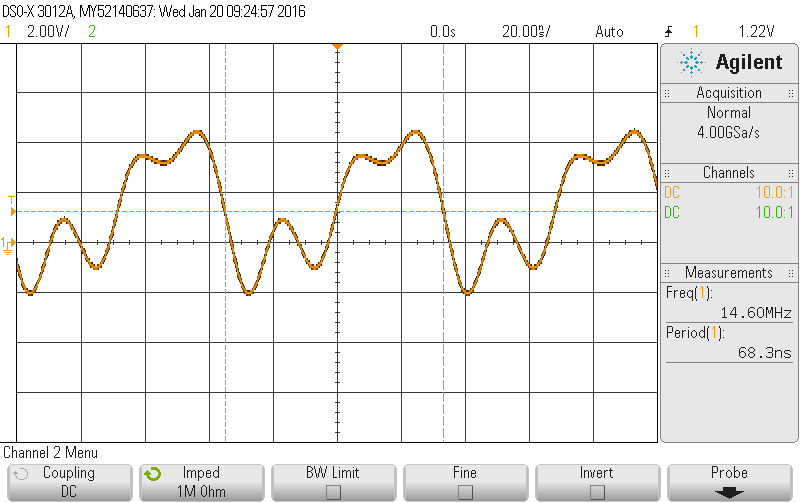
\includegraphics[width=\linewidth]{Practicum_1_Content/Part_iii/LSdeviceringosc.png}
    \caption{TTL Device Ring Oscillator Output}
\end{figure} %TTL ring oscillator output
\begin{table}[ht]
\caption{74LS04} % title of Table
\centering % used for centering table
\begin{tabular}{|c|c|c|c|c|}
\hline %inserts double horizontal lines
Parameter & Typ/Min & Max & Measured & Units\\ [0.5ex]
% inserts table
%heading
\hline % inserts single horizontal line
Period of oscillation & - & - & 68.3 & ns \\
Average propagation delay per gate & 4 & 15 & 22.8 & ns \\
Power dissipation per gate (@1MHz) & 3.64 & 3.64 &   & mW \\
Power-delay product & 14.56 & 54.6 &  & pW \\
Energy-delay product & ${5.824\times10^{-8}}$ & ${81.9\times10^{-8}}$ & & pJ \\ [1ex] % [1ex] adds vertical space
\hline %inserts single line
\end{tabular}
\label{table:nonlin} % is used to refer this table in the text
\end{table}
\begin{figure}
    \centering
    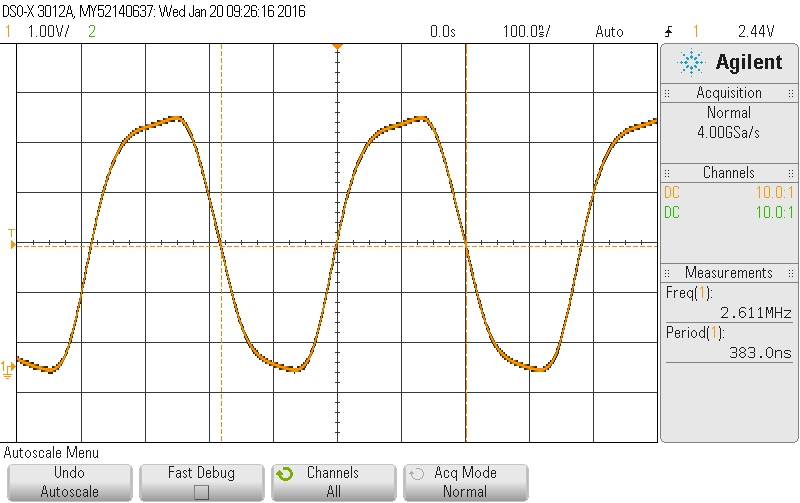
\includegraphics[width=\linewidth]{Practicum_1_Content/Part_iii/CMOSringosc.png}
    \caption{CMOS Ring Oscillator Output}
\end{figure}
\begin{table}[ht]
\caption{CMOS 4096} % title of Table
\centering % used for centering table
\begin{tabular}{|c|c|c|c|c|}
\hline %inserts double horizontal lines
Parameter & Typ/Min & Max & Measured & Units\\ [0.5ex]
% inserts table
%heading
\hline % inserts single horizontal line
Period of oscillation & - & - & 383 & ns \\
Average propagation delay per gate & 65 & 125 & 127.7 & ns \\
Power dissipation per gate (@1MHz) & 1.47 & 1.47 &   & mW \\
Power-delay product & 95.55 & 183.75 &  & pW \\
Energy-delay product & ${621\times10^{-8}}$ & ${2297\times10^{-8}}$ & & pJ \\ [1ex] % [1ex] adds vertical space
\hline %inserts single line
\end{tabular}
\label{table:nonlin} % is used to refer this table in the text
\end{table}
\subsection{Discussion of Results}
We observe that the 74LS04 has a smaller period of oscillation of $68.3 ns$ versus the CMOS 4096's $383 ns$.  Thus the period of oscillation per gate is smaller in the 74LS04 ($22.8 ns$) than the CMOS 4096 ($127.7 ns$).  Using equation 1.6, we can determine the expected period of oscillation per gate for each device.  For the 74LS04, $T = 2Nt_{p} = 2(3)(15 ns) = 90 ns$.  Since we used the maximum $t_{p}$ value of $15 ns$, we obtained the maximum T value.  Hence, the period of oscillation is significantly higher than what we measured ($68.3 ns$).  For the CMOS 4096 device, $T = 2Nt_{p} = 2(3)(65 ns) = 390 ns$.  Here, we used a typical value of $t_{p}$.  Thus, our measured value of the period of oscillation is much closer to the calculated one ($390 ns$ vs. $383 ns$).
\subsection{Conclusions}
Looking at Figures 1.8 and 1.9, we see that the 74LS04 produced a much more rough signal than the CMOS 4096, which produced a smoother sinusoid.  The TTL device had much higher frequency components in the output of the ring oscillator.  These ripples may indicate that the 74LS04 device is not the best choice in making a ring oscillator since its output is the least sinusoidal of the two devices.  Because we did not calculate the PDP or EDP using our results, we cannot comment on any discrepancies between the predicted and measured values.  However, we can say that the 74LS04 oscillates much faster (nearly 5 times as fast) than the CMOS 4096 device.
\subsection{Prelab}
\begin{figure}
    \centering
    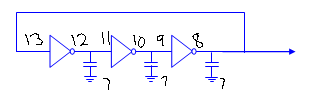
\includegraphics[width=\linewidth]{Practicum_1_Content/Part_iii/ringoscillatordiagram.png}
    \caption{Prelab Ring Oscillator Setup with Associated Pin Numbers}
\end{figure}
Refer to Table 1.7 and 1.8 for prelab values (predicted PDP and EDP values).



%%%%%%%%%%%%%%%
% PRACTICUM 2 %
%%%%%%%%%%%%%%%
\chapter{Practicum 2: Layout of a CMOS Circuit}
\section{Overview}
In this practicum, we use the Microwind software package to observe how a CMOS logic function could be laid out and implemented in fabrication.  CMOS, or complementary metal-oxide semiconductor, technology is ubiquitous in semiconductor technologies.  Since the CMOS is \textbf{complementary}, the layout of such a logic function contains complementary and symmetrical components of both p-type and n-type metal oxide semi conductor field effect transistors.
\section{Purpose}
This practicum is designed to further understand the layout of a CMOS circuit.  In addition, we gain the skill set of going from logic function to layout and layout to logic function.  This is an important skill to have so we can understand the behavior of a CMOS device by looking at its layout.
\section{Procedure}
Using the Microwind software package, the logic function $f = \overline{(a + b) \cdot (c + d)}$ was implemented.  In Microwind, we entered the Verilog code: $f = \sim((a|b)\&(c|d))$ in the \textbf{Compile} menu.  The compile button was pressed and the layout was generated.  We capture the layout as shown in Figure 2.2.  Next, we used the 2D and 3D tools in the \textbf{Simulate} menu to examine the circuit layout in further detail.  We capture both NMOS transistors and PMOS transistors in the 2D view (Figures 2.3 and 2.4).  Next, we return the \textbf{Simulate} menu again and select \textsc{Process Steps in 3D tool} to observe how the logic device can be fabricated.  We capture the 3D cross section in Figure 2.5).  Next, we construct the "stick diagram" of the CMOS circuit in MS Paint using Figure 2.2 as a reference.  This diagram is shown in Figure 2.6.  We then overlay the CMOS gates in Figure 2.7.
\section{Calculations, Data, and Graphs}
See figures.
\begin{figure}
    \centering
    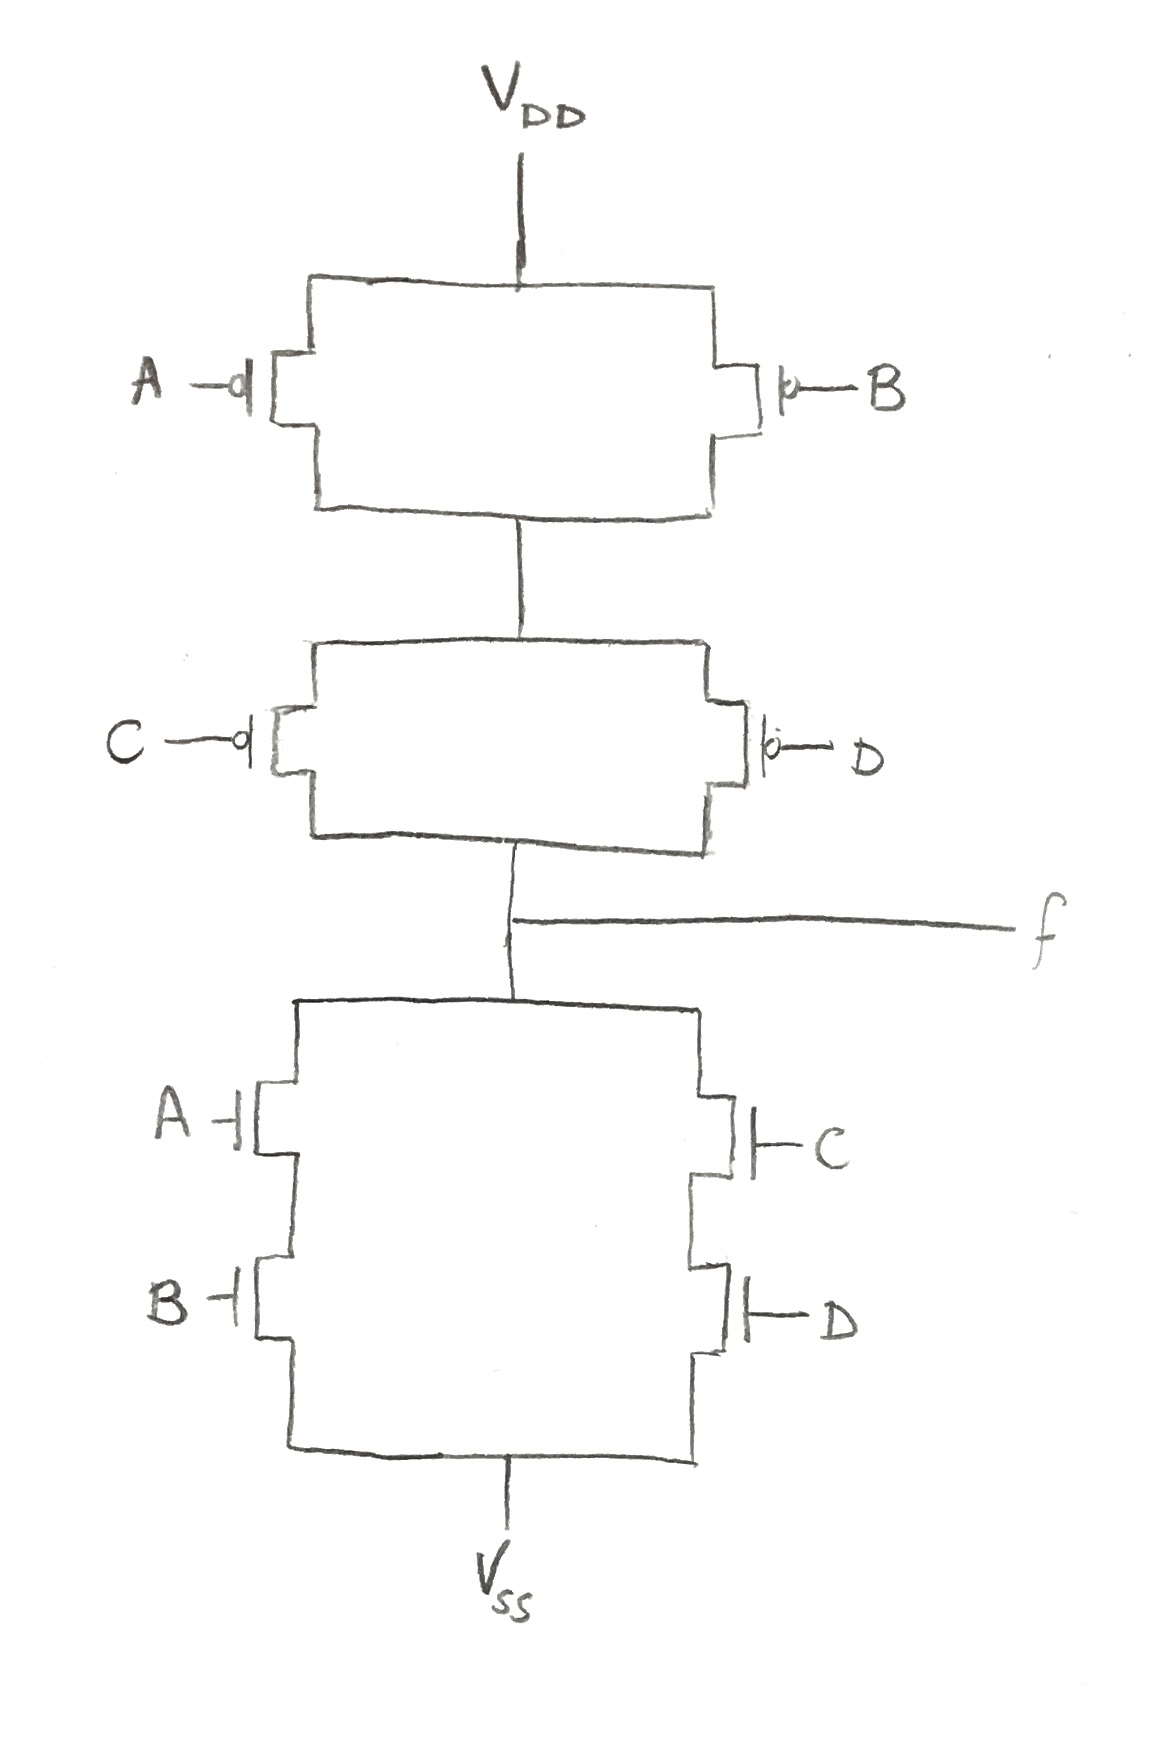
\includegraphics[width=\linewidth]{Practicum_2_Content/diagram.jpg}
    \caption{CMOS transistor layout of logic function}
\end{figure}
\begin{figure}
    \centering
    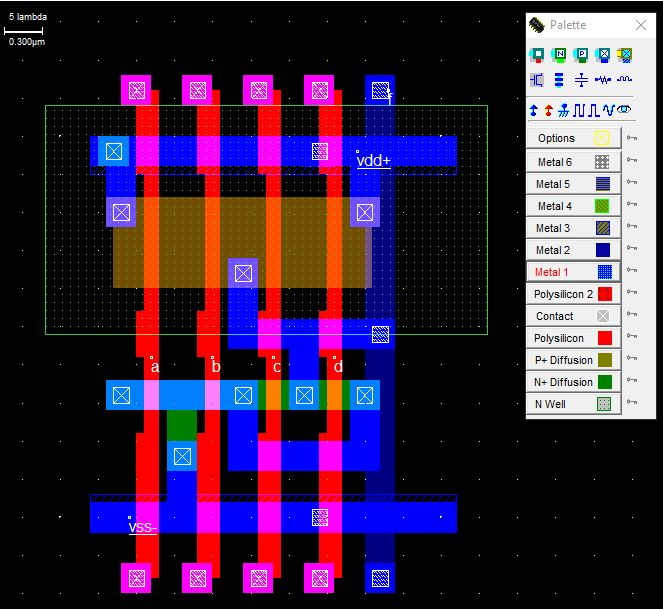
\includegraphics[width=\linewidth]{Practicum_2_Content/cmos_circuit_layout.JPG}
    \caption{Microwind layout of logic function}
\end{figure}
\begin{figure}
    \centering
    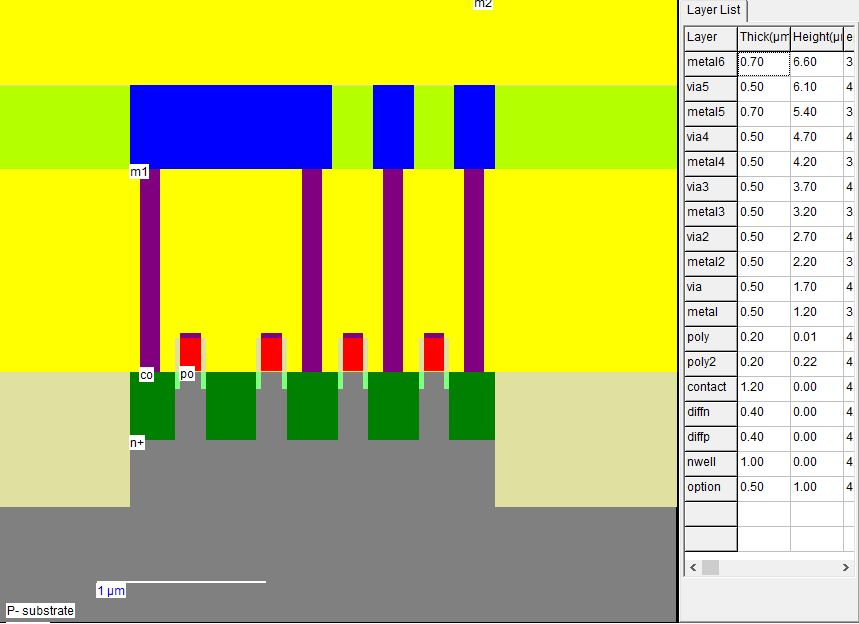
\includegraphics[width=\linewidth]{Practicum_2_Content/cmos_2d_nmos.JPG}
    \caption{2D cross-sectional view of NMOS transistors}
\end{figure}
\begin{figure}
    \centering
    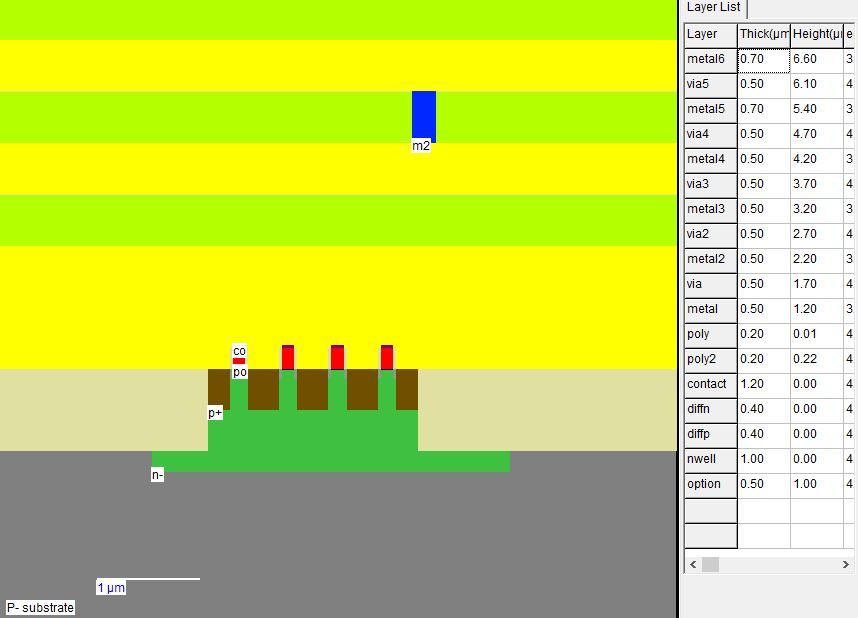
\includegraphics[width=\linewidth]{Practicum_2_Content/cmos_2d_pmos.JPG}
    \caption{2D cross-sectional view of PMOS transistors}
\end{figure}
\begin{figure}
    \centering
    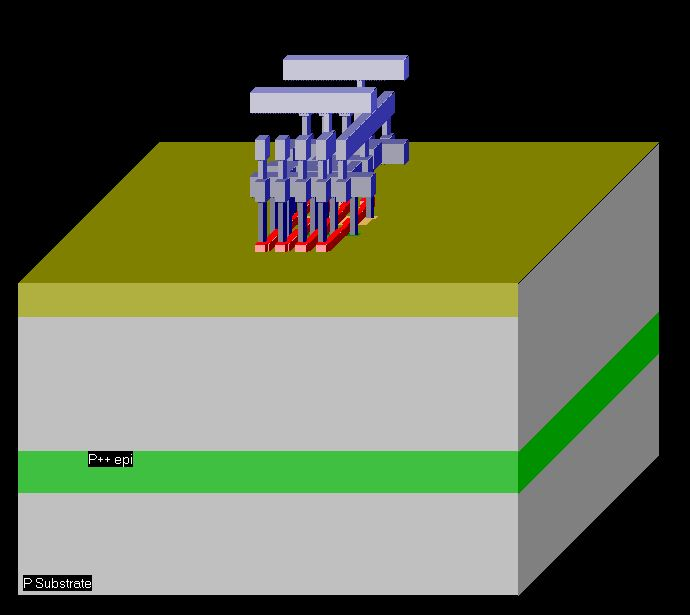
\includegraphics[width=\linewidth]{Practicum_2_Content/cmos_3d.JPG}
    \caption{3D view of CMOS circuit}
\end{figure}
\begin{figure}
    \centering
    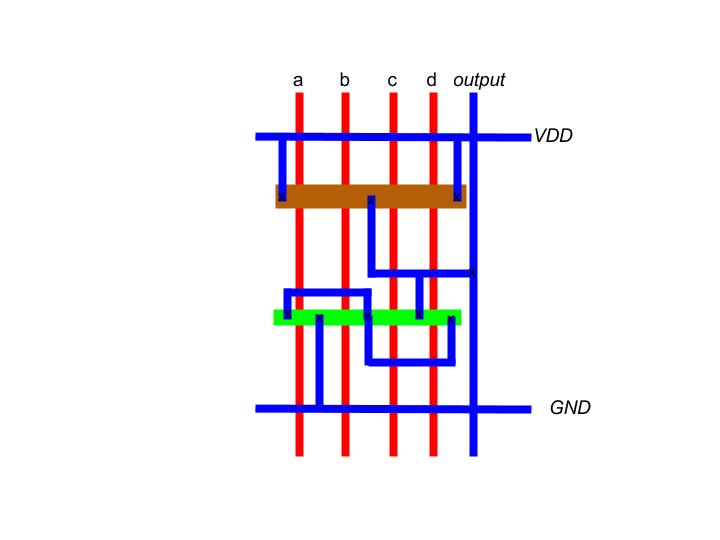
\includegraphics[width=\linewidth]{Practicum_2_Content/cmos_stick.jpg}
    \caption{Stick diagram of logic function}
\end{figure}
\begin{figure}
    \centering
    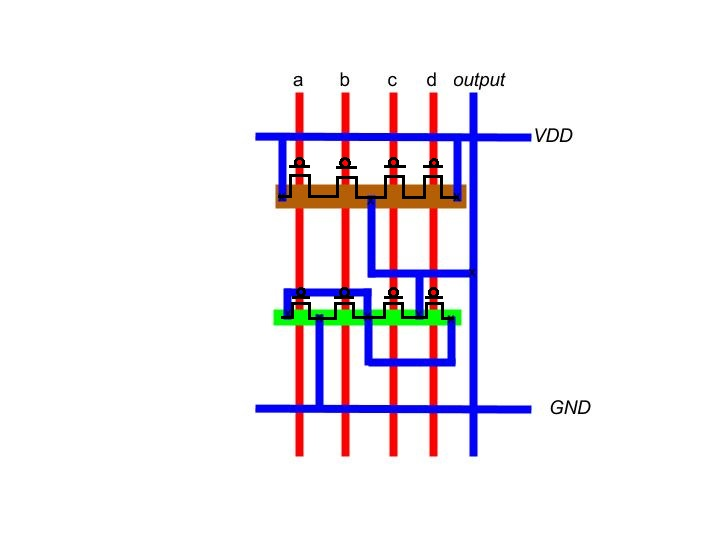
\includegraphics[width=\linewidth]{Practicum_2_Content/cmos_stick_transistors.jpg}
    \caption{Stick diagram of logic function with metal interconnects}
\end{figure}
\section{Discussion of Results}
We have thus shown that the logic function $f = \overline{(a + b) \cdot (c + d)}$ can be built using CMOS technology.  In Microwind, we can observe the fabrication steps needed to build such a device.  Using MS paint, we construct the stick diagram and locate the transistor locations for this logic function.
\section{Conclusions}
Microwind is a powerful and easy-to-use software that can be used to structure the layout of any logic function in CMOS gate technologies.  We successfully implemented the logic function $f = \overline{(a + b) \cdot (c + d)}$ in such a way that we can observe the fabrication steps and construct a stick diagram to make analysis easier.

%%%%%%%%%%%%%%%
% PRACTICUM 3 %
%%%%%%%%%%%%%%%
\chapter{Practicum 3: DE2 and Quartus Intro}
\section{Overview}
Altera Quartus II is a powerful tool to build, model, and test circuits.  Schematic capture and VHDL (VHSIC Hardware Description Language) are both important tools required to test characteristics of an ORing gate circuit in this practicum.
\section{Purpose}
The purpose of this practicum is to gain a basic understanding of how to use the Altera Quartus II CAD software package.  Using both schematic capture and VHDL, we can observe important characteristics in any circuit we design.
\section{Procedure}
\textbf{Part 1: Using Schematic Capture to Configure the Altera DE2 Board} \\
A USB cable was connected to the DE2 board and a USB port on a computer with Altera Quartus II CAD tools installed.  Then, the 9V DC transformer was connected to the DE2 board and plugged into a 120V AC outlet.  The ORing gate circuit was set up for the Cyclone II chip using pates 1-18 of the reference "\textit{Tutorial I: The 15-Minute Design}".  Next, the ORing gate circuit was uploaded to the Cyclone II chip on the DE2 board using pages 22-24 of the same reference. 

\textbf{Part 2: Using VHDL to Configure the Altera DE2 Board} \\
The procedures described in Part 1 were repeated using VHDL code using pages 29-33 as a reference.

\textbf{Part 3: Timing Analysis, Floorplan Editor, Symbol Creation, and Functional Simulation Tools} \\
Using pages 38-41 as a reference, a timing analysis was performed to determine the maximum delay in the ORing gate circuit on the Cyclone II chip.  Then, the floorplan editor was used to figure out the location of the ORing gate circuit on the Cyclone II chip.  The Chip Planner under the Tools menu was used.  Fan-in and fan-out tools were used to see the signal path delays between the LE and I/O circuits on the periphery of the Cyclone II chip.  Then, a symbol block was generated from the VHDL code.  And a functional simulation of the ORing gate circuit was performed.

\textbf{Part 4: Additional Exercises}\\
The chip editor was used to move the logic cell used in the ORing gate design to another location inside the Cyclone II chip.  It was moved several columns away from the pushbutton and LED pins.  The timing analyzer was run and compared to the original results.  Finally, the logic circuit designed in the prelab was used to turn on the LED when both pushbuttons were pressed.  The circuit was compiled, simulated, downloaded, and tested.
\section{Calculations, Data, and Graphs}
Refer to Figures 3.1-3.7.
\begin{figure}
    \centering
    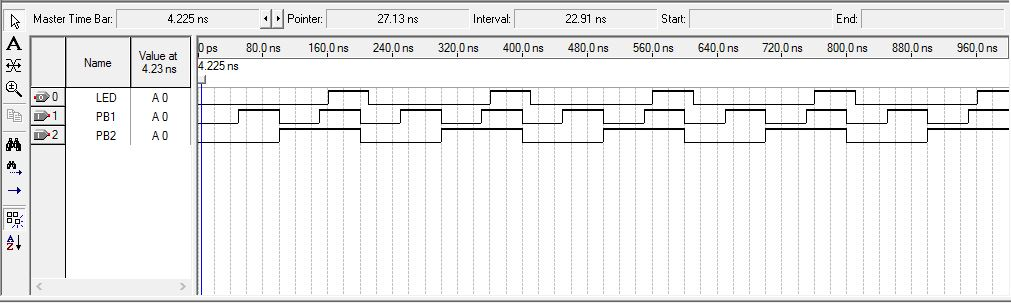
\includegraphics[width=\linewidth]{Practicum_3_Content/1_simulation_waveform.JPG}
    \caption{Part 1: Simulation Waveform}
\end{figure}
\begin{figure}
    \centering
    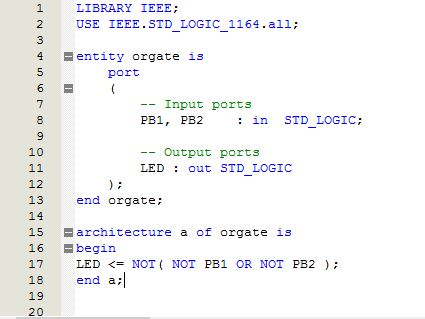
\includegraphics[width=\linewidth]{Practicum_3_Content/2_1_vhdl_code.JPG}
    \caption{Part 2: VHDL Code}
\end{figure}
\begin{figure}
    \centering
    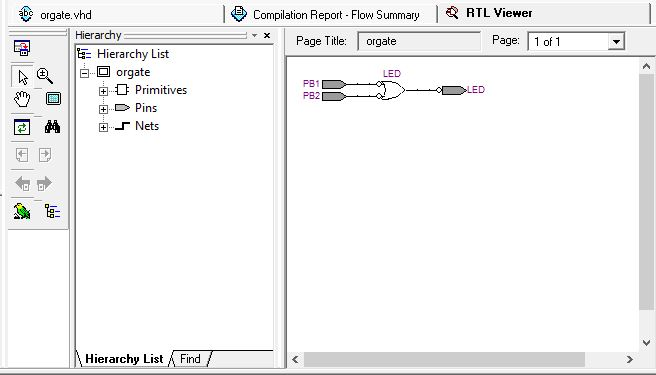
\includegraphics[width=\linewidth]{Practicum_3_Content/2_2_diagram_from_code}
    \caption{Part 2: Diagram From Code}
\end{figure}
\begin{figure}
    \centering
    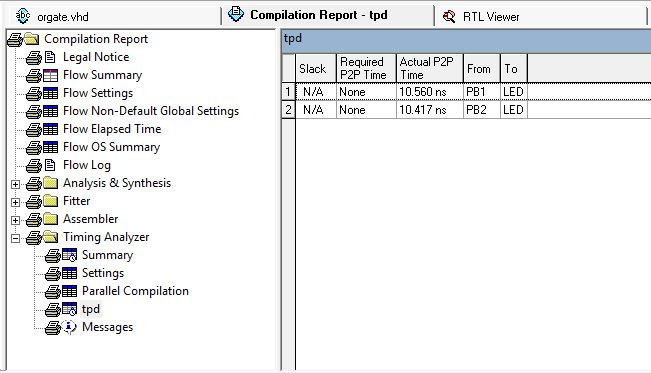
\includegraphics[width=\linewidth]{Practicum_3_Content/3_1_tpd.JPG}
    \caption{Part 3: Timing Analysis}
\end{figure}
\begin{figure}
    \centering
    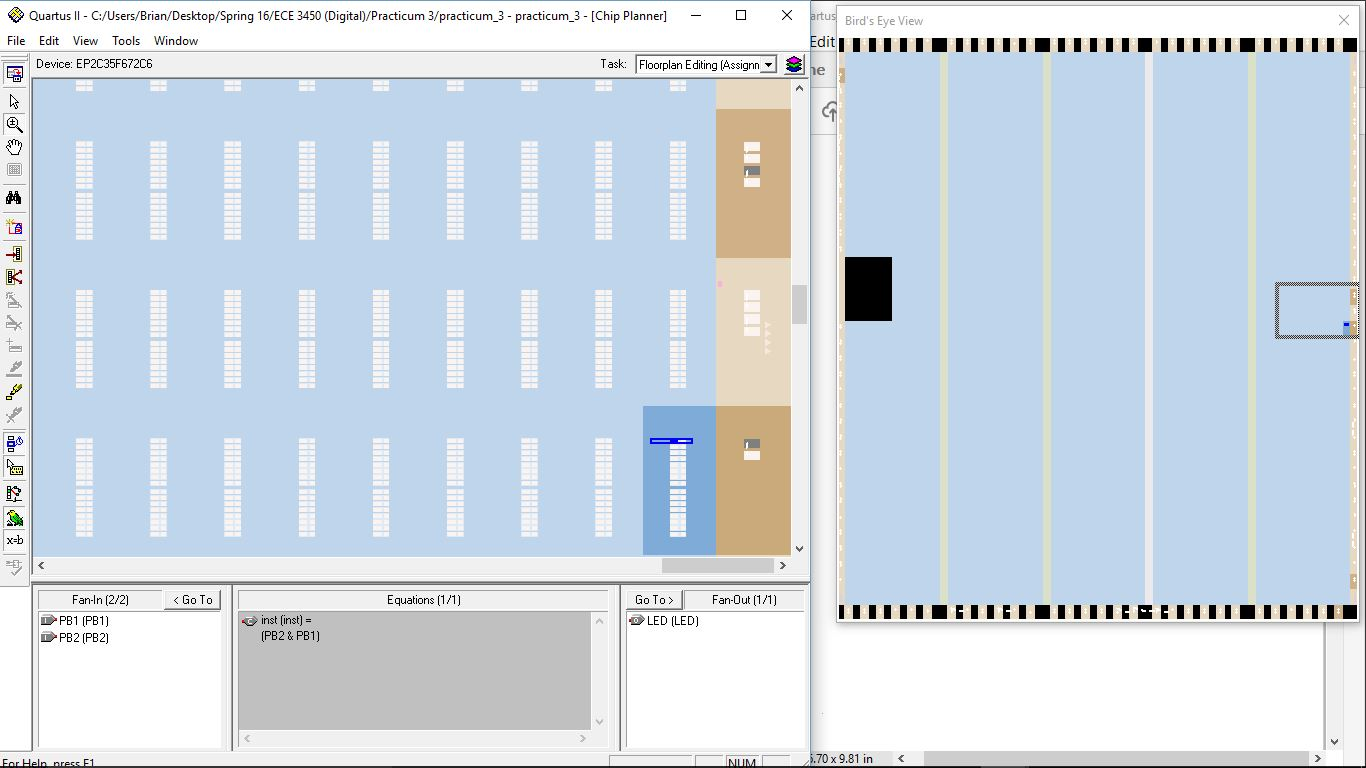
\includegraphics[width=\linewidth]{Practicum_3_Content/3_2_floorplan.JPG}
    \caption{Part 3: Floorplan}
\end{figure}
\begin{figure}
    \centering
    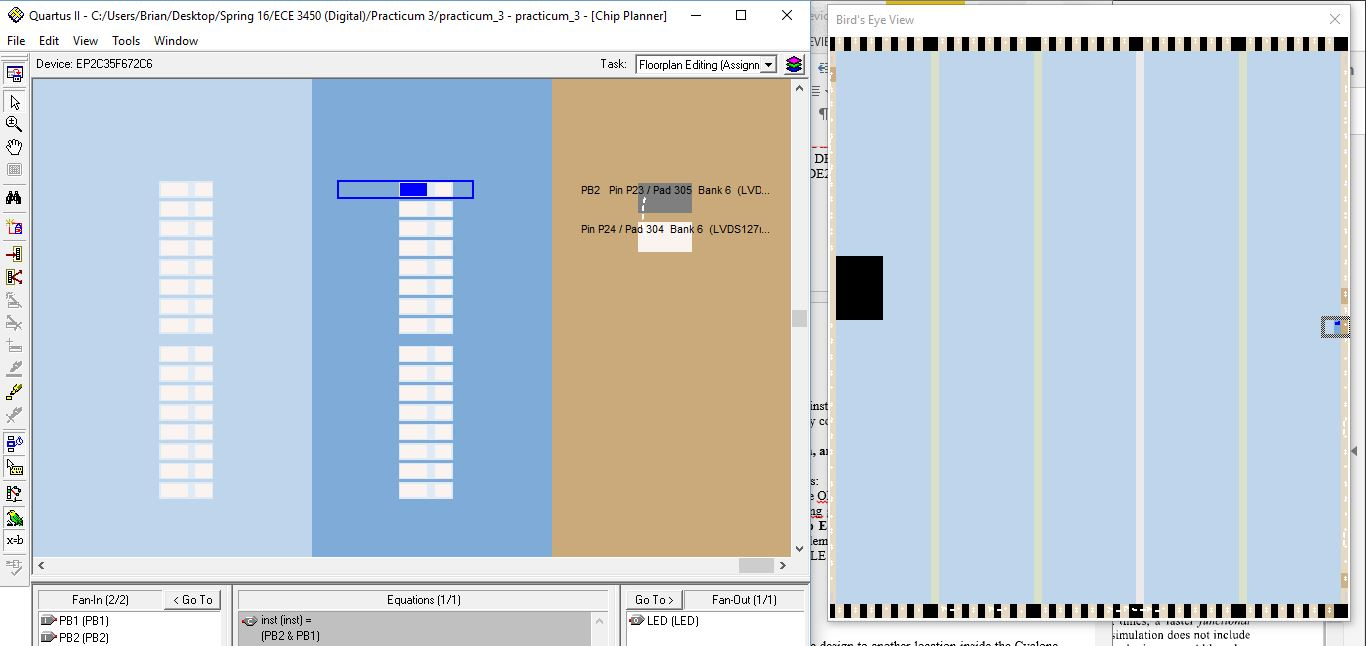
\includegraphics[width=\linewidth]{Practicum_3_Content/3_3_floorplan_zoom.JPG}
    \caption{Part 3: Closer View of Floorplan}
\end{figure}
\begin{figure}
    \centering
    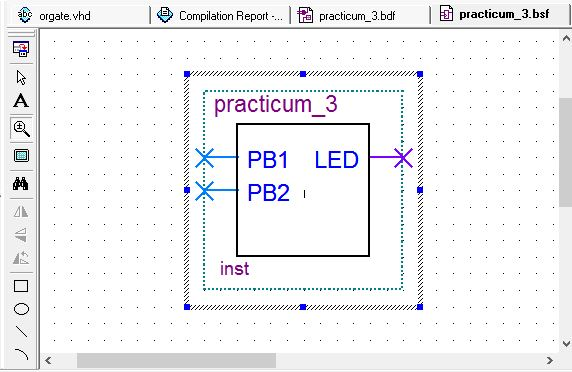
\includegraphics[width=\linewidth]{Practicum_3_Content/3_4_block_diagram.JPG}
    \caption{Part 3: Block Diagram}
\end{figure}
\section{Discussion of Results}
Using Altera Quartus II timing analysis the time delay from PB1 to the LED was 10.560ns and 10.417ns from PB2 to the LED.  These delays are virtually nonexistent since they are so small, us humans cannot even perceive the delay.  Moving the logic cell placement from the default to another location changed the delays to 12.212ns for PB1 to the LED and 12.561ns for PB2 to the LED.  Even with the larger delay times, this magnitude of delay is still unperceivable to us. 
\section{Conclusions}
This practicum served as the introduction to a powerful digital CAD tool, Altera Quartus II.  Each section of the lab was completed and documented successfully.  By successfully modeling an ORing gate (acting as an AND gate, specifically) and observing the timing behavior of the circuit, we can understand how logic placement on a chip can be very important.
\section{Prelab}
\begin{table}[ht]
\caption{Prelab: Truth Table for an "ORing gate" with active-low inputs connected to pushbuttons and an active-low output driving an LED} % title of Table
\centering % used for centering table
\begin{tabular}{|c|c|c|c|c|}
\hline %inserts double horizontal lines
PB1 & PB2 & OUT & LED (on or off)\\ [0.5ex]
% inserts table
%heading
\hline % inserts single horizontal line
0 & 0 & 0 & ON \\
0 & 1 & 0 & ON \\
1 & 0 & 0 & ON \\
1 & 1 & 1 & OFF \\ [1ex] % [1ex] adds vertical space
\hline %inserts single line
\end{tabular}
\label{table:nonlin} % is used to refer this table in the text
\end{table}


%%%%%%%%%%%%%%%
% PRACTICUM 4 %
%%%%%%%%%%%%%%%
\chapter{Practicum 4: VHDL Coding and Simulation Assignments}
\section{Overview}
In this practicum, VHDL (VHSIC Hardware Description Language) code was written in Altera Quartus II.  This code was then used to generate a timing diagram and TPD analyses.  VHDL is a powerful tool used to describe and analyze digital systems such as field programmable gate arrays (FPGAs) and integrated circuits.
\section{Purpose}
The purpose of this practicum is to gain a better understanding of coding in VHDL and performing timing diagram analyses.  In addition, by observing the TPDs of two different chips, we can observe how signals propagate through these chips.  Depending on the application, one chip may be preferable over another.
\section{Procedure}
The following problems were performed using Brown and Vranesic's textbook \textit{Fundamentals of Digital Logic with VHDL Design $3^{rd}$ Edition}.
\begin{enumerate}
  \item Problem 2.52 on page 74. A functional simulation in Altera Quartus II was used to verify.
  \item Problem 3.51 a and b on page 164. Quartus II was used to observe the timing simulation.  A critical path (the signal path with the longest propagation delay) was found in the circuit.  For \textbf{Part a}, the Max 7000S CPLD (EPM7128SLC84-7) was used.  For \textbf{Part b}, the Cyclone II FPGA (EP2C35F672C6) was used.
  \item Problem 4.45 on page 245.  A functional simulation in Quartus II was performed to verify.
  \item Problem 5.16b on page 313.  A functional simulation in Quartus II was performed to verify.
  \item Problem 7.10 on page 478.  A functional simulation in Quartus II was performed to verify.
\end{enumerate}
The following problems were individual assignments performed outside of class:
\begin{enumerate}
  \item Problem 2.51 on page 74.  A functional simulation in Quartus II was performed to verify.
  \item Problem 3.52 a and b on page 164.  Quartus II was used to observe the timing simulation.  A critical path (the signal path with the longest propagation delay) was found in the circuit.  For \textbf{Part a}, the Max 7000S CPLD (EPM7128SLC84-7) was used.  For \textbf{Part b}, the Cyclone II FPGA (EP2C35F672C6) was used.
  \item Problem 4.47 on page 245.  A functional simulation in Quartus II was performed to verify.
  \item Problem 5.16a on page 313.  A functional simulation in Quartus II was performed to verify.
  \item Problem 7.11 on page 478.  A functional simulation in Quartus II was performed to verify.
\end{enumerate}

\section{Calculations, Data, and Graphs}
Refer to figures.
\begin{figure}
    \centering
    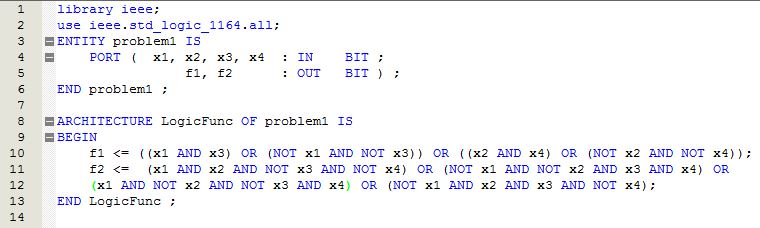
\includegraphics[width=\linewidth]{Practicum_4_Content/inlab/1_1_code.JPG}
    \caption{Laboratory Part 1 (Problem 2.52) Code}
\end{figure}
\begin{figure}
    \centering
    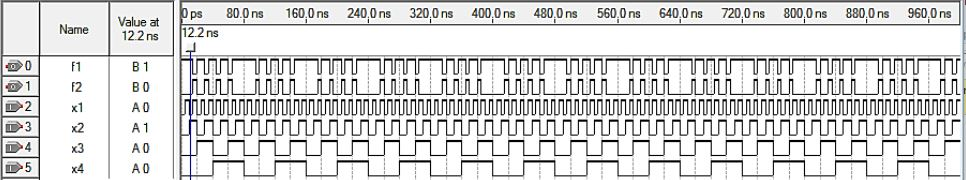
\includegraphics[width=\linewidth]{Practicum_4_Content/inlab/1_2_time.JPG}
    \caption{Laboratory Part 1 (Problem 2.52) Timing Diagram}
\end{figure}
\begin{figure}
    \centering
    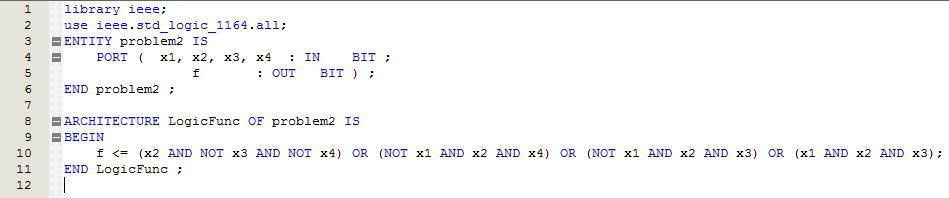
\includegraphics[width=\linewidth]{Practicum_4_Content/inlab/2_1_code.JPG}
    \caption{Laboratory Part 2 (Problem 3.51) Code}
\end{figure}
\begin{figure}
    \centering
    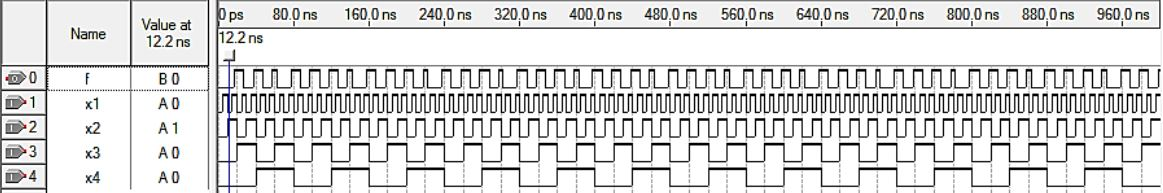
\includegraphics[width=\linewidth]{Practicum_4_Content/inlab/2_2_time.JPG}
    \caption{Laboratory Part 2 (Problem 3.51) Timing Diagram}
\end{figure}

%%place two figures side by side
\begin{figure}[!htb]
\minipage{0.45\textwidth}
  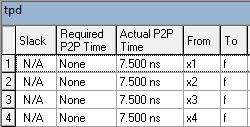
\includegraphics[width=\linewidth]{Practicum_4_Content/inlab/2_3_tdp_MAX.JPG}
  \caption{Laboratory Part 2 (Problem 3.51) TPD Using Max 7000S Chip}
\endminipage\hfill
\minipage{0.45\textwidth}
  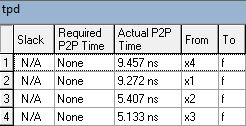
\includegraphics[width=\linewidth]{Practicum_4_Content/inlab/2_4_tpd_cyclone2.JPG}
  \caption{Laboratory Part 2 (Problem 3.51) TPD Using Cyclone II Chip}
\endminipage
\end{figure}

\begin{figure}
    \centering
    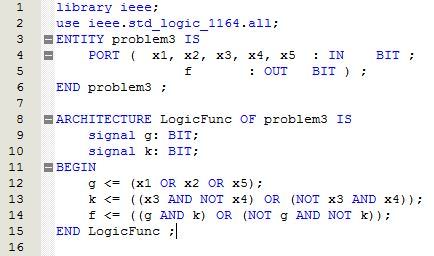
\includegraphics[width=\linewidth]{Practicum_4_Content/inlab/3_1_code.JPG}
    \caption{Laboratory Part 3 (Problem 4.47) Code}
\end{figure}
\begin{figure}
    \centering
    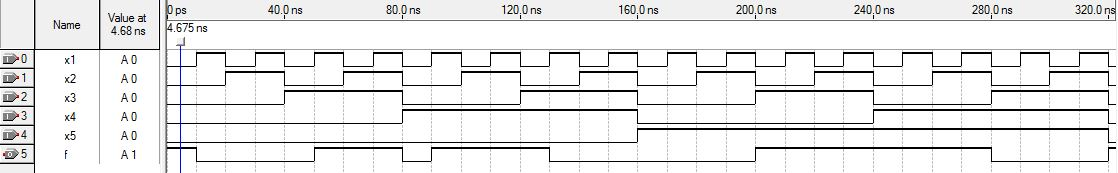
\includegraphics[width=\linewidth]{Practicum_4_Content/inlab/3_2_time.JPG}
    \caption{Laboratory Part 3 (Problem 4.47) Timing Diagram}
\end{figure}

\begin{figure}
    \centering
    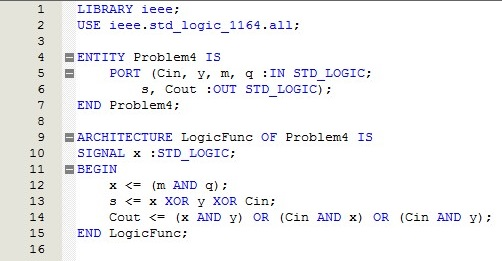
\includegraphics[width=\linewidth]{Practicum_4_Content/inlab/4_1_code.jpg}
    \caption{Laboratory Part 4 (Problem 5.16b) Code}
\end{figure}
\begin{figure}
    \centering
    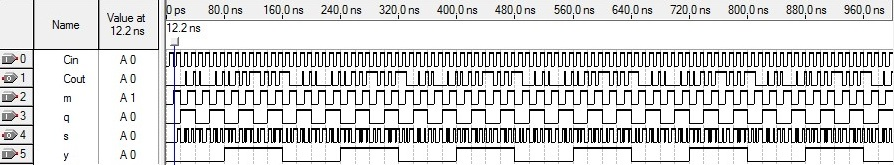
\includegraphics[width=\linewidth]{Practicum_4_Content/inlab/4_2_time.jpg}
    \caption{Laboratory Part 4 (Problem 5.16b) Timing Diagram}
\end{figure}

\begin{figure}
    \centering
    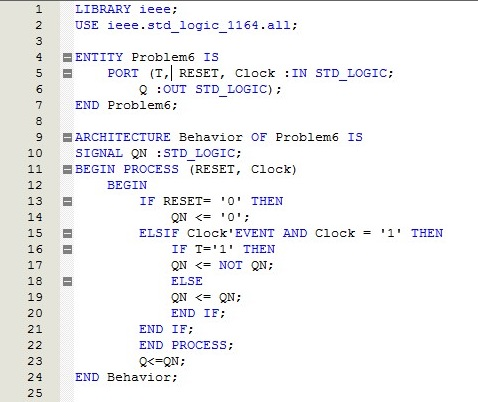
\includegraphics[width=\linewidth]{Practicum_4_Content/inlab/5_1_code.jpg}
    \caption{Laboratory Part 5 (Problem 7.10) Code}
\end{figure}
\begin{figure}
    \centering
    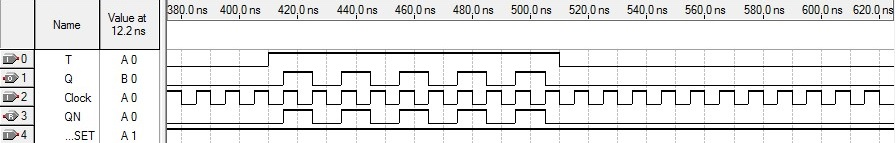
\includegraphics[width=\linewidth]{Practicum_4_Content/inlab/5_2_time.jpg}
    \caption{Laboratory Part 5 (Problem 7.10) Timing Diagram}
\end{figure}
\begin{figure}
    \centering
    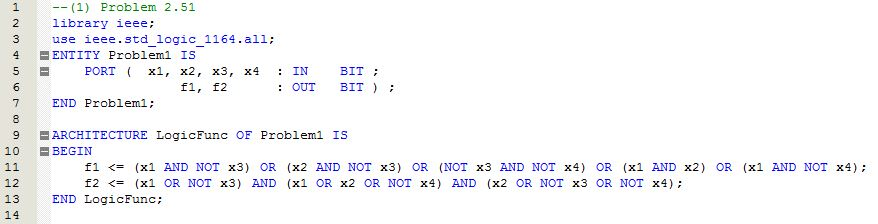
\includegraphics[width=\linewidth]{Practicum_4_Content/Homework/1_1_code.JPG}
    \caption{Homework Part 1 (Problem 2.51) Code}
\end{figure}
\begin{figure}
    \centering
    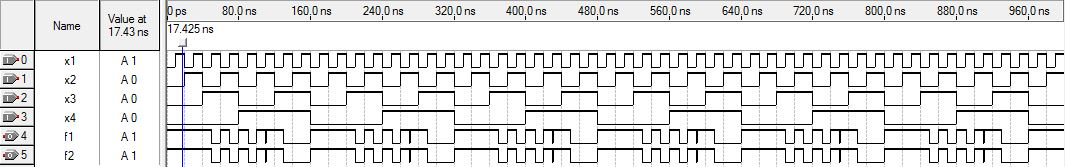
\includegraphics[width=\linewidth]{Practicum_4_Content/Homework/1_2_time.JPG}
    \caption{Homework Part 1 (Problem 2.51) Timing Diagram}
\end{figure}
\begin{figure}
    \centering
    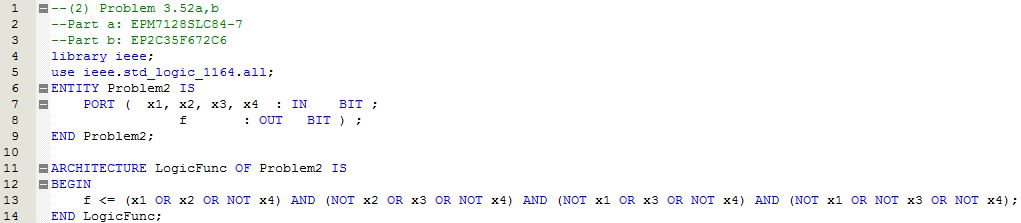
\includegraphics[width=\linewidth]{Practicum_4_Content/Homework/2_1_code.JPG}
    \caption{Homework Part 2 (Problem 3.52) Code}
\end{figure}
\begin{figure}
    \centering
    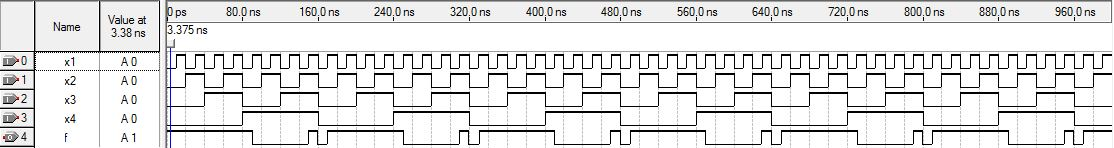
\includegraphics[width=\linewidth]{Practicum_4_Content/Homework/2_2_time.JPG}
    \caption{Homework Part 2 (Problem 3.52) Timing Diagram}
\end{figure}



%%place two figures side by side
\begin{figure}[!htb]
\minipage{0.45\textwidth}
  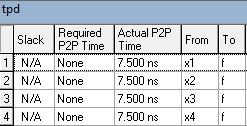
\includegraphics[width=\linewidth]{Practicum_4_Content/Homework/2_3_tpd_max.JPG}
  \caption{Homework Part 2 (Problem 3.52) TPD Using Max 7000S Chip}
\endminipage\hfill
\minipage{0.45\textwidth}
  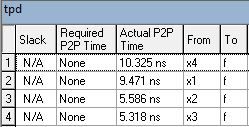
\includegraphics[width=\linewidth]{Practicum_4_Content/Homework/2_4_tpd_cyclone.JPG}
  \caption{Homework Part 2 (Problem 3.52) TPD Using Cyclone II Chip}
\endminipage
\end{figure}


\begin{figure}
    \centering
    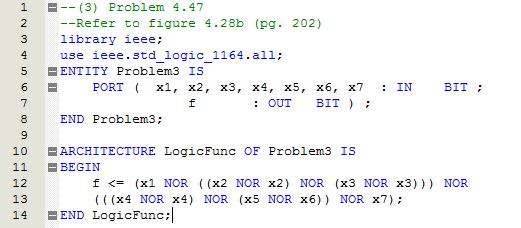
\includegraphics[width=\linewidth]{Practicum_4_Content/Homework/3_1_code.JPG}
    \caption{Homework Part 3 (Problem 4.47) Code}
\end{figure}
\begin{figure}
    \centering
    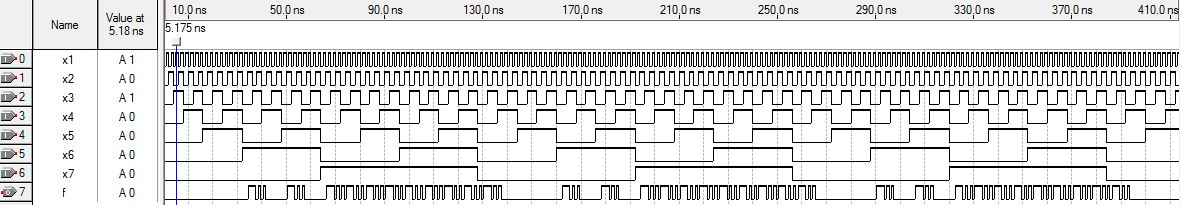
\includegraphics[width=\linewidth]{Practicum_4_Content/Homework/3_2_time.JPG}
    \caption{Homework Part 3 (Problem 4.47) Timing Diagram}
\end{figure}
\begin{figure}
    \centering
    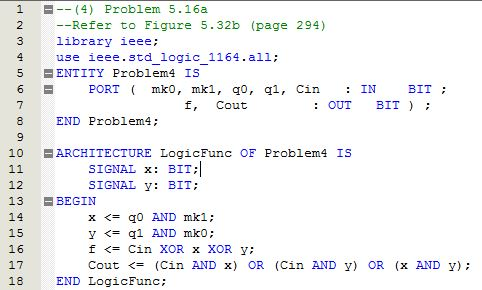
\includegraphics[width=\linewidth]{Practicum_4_Content/Homework/4_1_code.JPG}
    \caption{Homework Part 4 (Problem 5.16a) Code}
\end{figure}
\begin{figure}
    \centering
    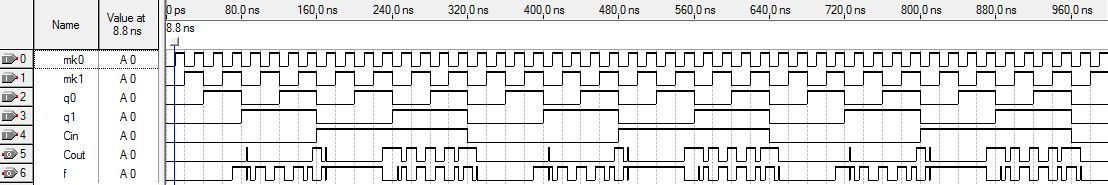
\includegraphics[width=\linewidth]{Practicum_4_Content/Homework/4_2_time.JPG}
    \caption{Homework Part 4 (Problem 5.16a) Timing Diagram}
\end{figure}
\begin{figure}
    \centering
    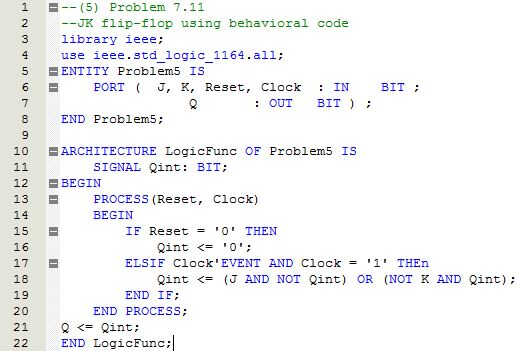
\includegraphics[width=\linewidth]{Practicum_4_Content/Homework/5_1_code.JPG}
    \caption{Homework Part 5 (Problem 7.11) Code}
\end{figure}
\begin{figure}
    \centering
    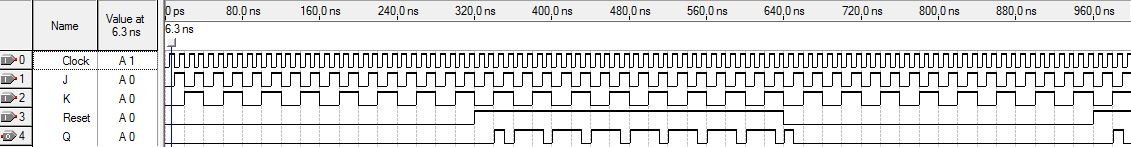
\includegraphics[width=\linewidth]{Practicum_4_Content/Homework/5_2_time.JPG}
    \caption{Homework Part 5 (Problem 7.11) Timing Diagram}
\end{figure}
\section{Discussion of Results}

\large{\textbf{Laboratory}}
\begin{enumerate}
  \item Problem 1: f1 and f2 appear to be the complement of each other.
  \item Problem 2: The MAX 7000S device exhibited a propagation delay of 7.5 ns whereas the Cyclone II FPGA had a range of propagation delays.  The Cyclone II had the smallest propagation delay (5.133 ns), but it also had the largest (9.457 ns).
  \item Problem 3: Problem 3 involved a series of logic gates.
  \item Problem 4: Here, we observe 'Cout,' the ORing of 3 AND gates.
  \item Problem 5: In this problem we have to define a 'Behavior' structure and a process with a reset and clock.
\end{enumerate}
\large{\textbf{Homework}}
\begin{enumerate}
  \item Problem 1: Observing the VHDL code, f1 and f2 look like very different logic functions.  However, when we run the simulation, we see that f1 and f2 exhibit the same behavior.  Using DeMorgan’s Laws, we can prove again that the two logic functions are the same.
  \item Problem 2: The MAX 7000S device exhibited a propagation delay of 7.5 ns whereas the Cyclone II FPGA had a range of propagation delays.  The Cyclone II had the smallest propagation delay (5.318 ns), but it also had the largest (10.325 ns).
  \item Problem 3: Problem 3 involved a series of NOR gates to produce a single output ‘f.’  
  \item Problem 4: Here, we observe ‘f’, the output of the full adder in a segment of a 4x4 multiplier circuit and ‘Cout,’ the carry bit output of the full adder.
  \item Problem 5: We notice that when ‘Reset’ has a logic state ‘high,’ output ‘Q’ exhibits JK flip-flop behavior as shown in lines 15-18 of the code.  When ‘Reset’ has a logic state ‘low,’ ‘Q’ remains at logic state ‘low.’  However, when ‘Reset’ toggles from ‘high’ to ‘low,’ ‘Q’ has a logic state ‘high’ until ‘J’ toggles ‘high.’
\end{enumerate}

\section{Conclusions}
Each problem involved VHDL coding and a timing analysis.  These steps were performed successfully.  Problem 2 in both the laboratory and homework sections involved two TPD analyses using two different chips: the MAX 7000S and the Cyclone II.  From these simulations, we can observe how long signals take to propagate in each chip.  Depending on the application, one chip may be preferable over the other.  VHDL is a powerful, yet challenging, tool.  It can be used to describe a logical circuit without building it.  By observing the behavior of the circuit specified by VHDL code, we can make accurate predictions about how the physical circuit will behave.

%%%%%%%%%%%%%%%
% PRACTICUM 5 %
%%%%%%%%%%%%%%%
\chapter{Practicum 5: Capacitance Sensor Project}
\section{Overview}
In this report, we will discuss two different implementations of a capacitance sensor: one using a Altera DE2 Development and Education Board in conjunction with Altera's Quartus II and the other using an Arduino.  

To measure the capacitance of a given capacitor, we can measure the period of the output of a capacitor with an input clock signal.  Because of the nature of a capacitor, the period is directly proportional to the capacitance.  So, the higher the capacitance, the higher the period is.  To measure the period, both implementations use a 555 timer (further detailed in Section 2: Design).  Then, the job of the DE2 and Arduino is to parse the output of the 555 timer into something useful for us humans.  Specifically, we have the DE2 board display the period on two of its seven segment LED displays.  With the Arduino, we have the period displayed on the serial monitor in the Arduino application.  If the period exceeds the range of the seven segment displays on the DE2 ($> 99$), we implement an offset feature to subtract powers of 2 from the output so that the display reads a value less than 99.  To obtain the final period, we just need to add the offset value to the displayed value.  This feature is implemented in the Arduino capacitance sensor in the form of a potentiometer. 

In the sections that follow, we will run through the designs, simulations, and testing \& verification of both the DE2 and Arduino implementations.

\section{Design}
In this section, we provide details on both the DE2-based design and the Arduino-based designs.

\subsection{DE2}
Our capacitance sensor had to meet a certain number of specifications.  For instance, we needed to specify the maximum capacitance that our sensor can measure: $$C_{max} =  4C_{min}$$

We chose $C_{min} = 0.1 \mu F$ and specified a clock frequency $f_{clk} $ of 10 KHz.  We chose 10KHz because we did not want the clock to be too fast in the case of 100KHz or too slow in the case of 1 KHz.  We decided that 10KHz would be a good middle-ground. In the calculations below, we solve for $\Delta T$, the range of periods we can measure due to our $\Delta C$ range of capacitor values we can measure with our sensor.  We also solve for resistor values $R_{A}$ and $R_{B}$ that we need in our 555 timer circuit.

\begin{figure}
    \centering
    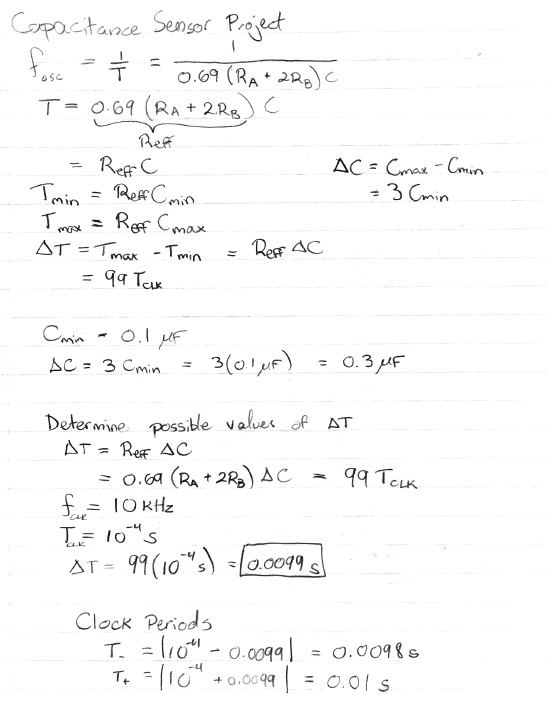
\includegraphics[width=\linewidth]{Practicum_5_Content/DE2/Calculations_1.jpg}
    \caption{Calculations for DE2 1/2}
\end{figure}
\begin{figure}
    \centering
    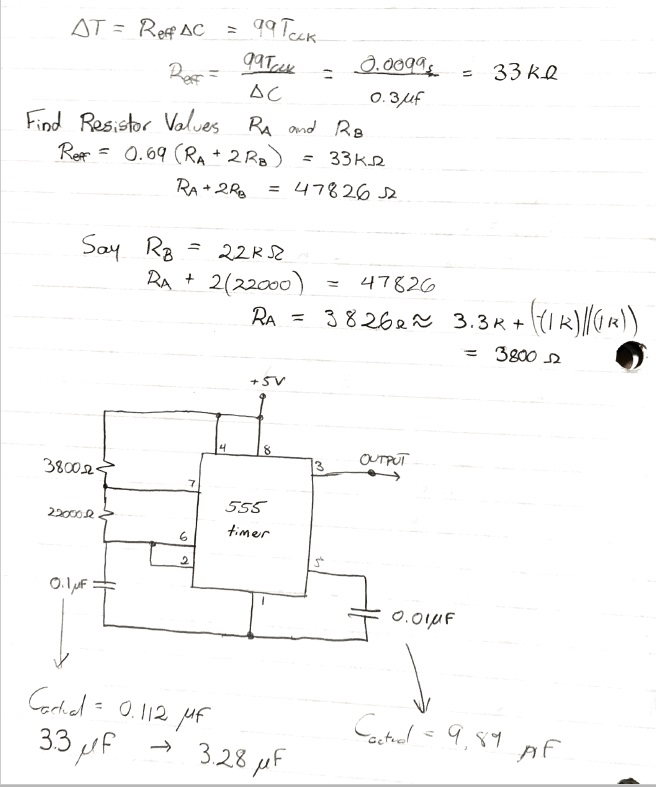
\includegraphics[width=\linewidth]{Practicum_5_Content/DE2/Calculations_2.jpg}
    \caption{Calculations for DE2 2/2}
\end{figure}


The overall block diagram of our DE2 implementation of the capacitance sensor is as follows.

\begin{figure}
    \centering
    \includegraphics[width=\linewidth]{Practicum_5_Content/DE2/blockDiagram.JPG}
    \caption{Block Diagram of the DE2 Capacitance Sensor}
\end{figure}
\begin{figure}
    \centering
    \includegraphics[width=\linewidth]{Practicum_5_Content/DE2/capsensor2bdf.jpg}
    \caption{Block Diagram of the DE2 Capacitance Sensor in Altera Quartus II}
\end{figure}

The 555 timer serves as the timer circuit that does the measuring of the capacitance.  This block in the diagram is a physical circuit and will thus not be coded for later on.  The divide by 2 circuit is a JK flipflop that transforms the output of the 555 timer circuit's period to twice that (from period T to 2T).  The 50 MHz oscillator on the DE2 board feeds in to the CLK\_DIV block, which gives us our operating frequency of 10KHz.  That 10KHz clock signal is then fed into our TIMER COUNT block.  This TIMER\_COUNT block measures the change of period ($\Delta T$) of oscillation due to the capacitor.  The 555 timer The period and capacitance are in a direct relationship so any positive change in the capacitance will result in a positive change in the period.  Likewise, a negative change in the capacitance will result in a negative change in the period of oscillation.  The multiplexer (or adder) block, reads in binary values set by the switches and subtracts that value from the output of the TIMER\_COUNT block.  For instance, if the capacitance is so large the period exceeds 99 on the displays (let us say it is 135), we can subtract 64 to get 71.  The offset switches are layed out in decreasing powers of two.  Reading from left to right the switches subtract $2^8, 2^7, 2^6, 2^5, 2^4, 2^3, 2^2, 2^1, 2^0$.  Having two or more switches in the on position will add the powers and subtract them from the TIMER\_COUNT output. The decoder is used to convert the binary from the output of the adder into the seven different segments in the seven segment display.  The reset button resets the values displayed on the seven segment displays (SEVEN\_SEG\_DISPLAY)

The CLK\_DIV, TIMER\_COUNT, adder, SEVEN\_SEG\_DISPLAY, and DEC 7SEG blocks were written in VHDL using Altera Quartus II.  The code for each block is listed in the Appendix.  The overall block diagram for the capacitance sensor is shown below.

\subsection{Arduino}
Using the same specifications from the DE2 implementation, we use the Arduino to replace the DE2 board.  This requires all coding in the Arduino application since we keep the same 555 timer circuit.  The only change we need to make is the offset voltage (as seen in figure 5).  This offset voltage is the same concept as the switches in the DE2 implementation.  We us a potentiometer to control the voltage reaching the Arduino.  If the period reading is over 99 we set the offset voltage to a value such that we do not have overflow (in the range of 00 to 99).  The reset button functionality is built in the Arduino.  So, pressing the reset button restarts the program.

\begin{figure}
    \centering
    \includegraphics[width=\linewidth]{Practicum_5_Content/Arduino/blockDiagram.JPG}
    \caption{Arduino Block Diagram}
\end{figure}

\begin{figure}
    \centering
    \includegraphics[width=\linewidth]{Practicum_5_Content/Arduino/pin_layout.JPG}
    \caption{Arduino Pin Layout}
\end{figure}

The Arduino sketch used for the capacitance sensor is listed in the Appendix.  We set the timer\_pin to pin 13 and the initial value of the offset to 0.  The offset value is then read from analog pin A0.  The duty cycle of the 555 timer is $\frac{2}{3}$ or approximately 0.67.  We then assign the clock period in microseconds.  Our clock frequency is 10KHz, so we set the period to 100 $\mu s$.  Then, we initialize the count values to 0 (in the same fashion as in the DE2 TIMER\_COUNT VHDL implementation). We define helper functions setup(), meas\_period(), and output\_value().  setup() defines the pin mode to use pin 13 as the input.  meas\_period() sets the pulse duration to the length of the pulse it reads from pin 13 (from the 555 timer circuit).  Because the pulse has a duty cycle of 0.67, we can use this fact to calculate the period of the signal.  Just like we did in the DE2 implementation, we only read out the maximum period the sensor measures.  The output\_value() function reads the offset value from the potentiometer and subtracts it from the count\_final variable we define as the period of the signal in the meas\_period() function.  Then, in the main loop, we perform meas\_period() and output\_value() and print out the period measured in meas\_period(), the offset, and the output value (with offset).  These values are output to the serial monitor in the Arduino application.  We can then observe the present values and compare them to past values the sensor reads.


%%%%
%%%%
%%%%

\section{Simulation}
In this section, we will discuss the simulation results of the DE2 implementation of the sensor.  The Arduino sensor did not have a simulation and thus will not be discussed here.

To test our DE2 capacitance sensor, we created a vector waveform file in Altera Quartus II.  This waveform had four inputs (Reset, CLK, input, and Offset) and three outputs (input\_2x, cout, and Output).  The reset was set high so that all of our values would not be set to 0.  Our clock CLK was set at 10KHz as described before.  The input was a square pulse train that halved its period partway through the simulation.  Our offset was set to 33 so that the maximum cout value would be 99.  The output maximum value would then be $cout - offset = 99 - 33 = 66$.  This is observed when the period of the input signal is halved.  Before it is halved, however, the cout period is 59 and thus $cout - offset = 59 - 33 = 26$.  This is seen from approximately 0ps to 130ms in the simulation.  From these results, we can conclude that our capacitance sensor does what we want it to do and we can begin testing and verifying the design.

\begin{figure}
    \centering
    \includegraphics[width=\linewidth]{Practicum_5_Content/DE2/Simulation/vector_waveform.PNG}
    \caption{Vector waveform from simulation of sensor}
\end{figure}

\section{Testing and Verification}
\subsection{DE2}
To test the sensor, we used various capacitors ranging from $C_{min} = 0.1 \mu F$ to $0.43 \mu F$.  The oscilloscope displays in Figures 9-14 are the outputs from the 555 timer with the specified capacitor values.  The table in Figure 15 summarizes the results obtained through the seven segment displays on the DE2 board (Output Values on DE2 Board column) as well as the measured periods from the oscilloscope (Period T column).


\begin{figure}[!htb]
\minipage{0.45\textwidth}
  \includegraphics[width=\linewidth]{Practicum_5_Content/DE2/01uF/01uF_555_Timer_output.jpg}
  \caption{$0.1 \mu F$ 555 timer output}
\endminipage\hfill
\minipage{0.45\textwidth}
  \includegraphics[width=\linewidth]{Practicum_5_Content/DE2/022uF/022uF_555_Timer_output.jpg}
  \caption{$0.22 \mu F$ 555 timer output}
\endminipage
\end{figure}

\begin{figure}[!htb]
\minipage{0.45\textwidth}
  \includegraphics[width=\linewidth]{Practicum_5_Content/DE2/032uF/032uF_555_Timer_output.jpg}
  \caption{$0.32 \mu F$ 555 timer output}
\endminipage\hfill
\minipage{0.45\textwidth}
  \includegraphics[width=\linewidth]{Practicum_5_Content/DE2/033uF/033uF_555_Timer_output.jpg}
  \caption{$0.33 \mu F$ 555 timer output}
\endminipage
\end{figure}


\begin{figure}[!htb]
\minipage{0.45\textwidth}
  \includegraphics[width=\linewidth]{Practicum_5_Content/DE2/041uF/041uF_555_Timer_output.jpg}
  \caption{$0.41 \mu F$ 555 timer output}
\endminipage\hfill
\minipage{0.45\textwidth}
  \includegraphics[width=\linewidth]{Practicum_5_Content/DE2/043uF/043uF_555_Timer_output.jpg}
  \caption{$0.43 \mu F$ 555 timer output}
\endminipage
\end{figure}

\begin{figure}
    \centering
    \includegraphics[width=\linewidth]{Practicum_5_Content/DE2/Results/tableOfResults.JPG}
    \caption{Summary of our measurements with different capacitors}
\end{figure}

In the Output Values on DE2 Board column of Figure 5.14, we write the period as a sum of two values if it exceeds 99.  The first values are the offsets subtracted using the switches and the second value is the reading on the seven segment displays after subtracting said value.  Adding the two results in the overall period.

We used Altera Quartus II's Signal Tap feature to test our sensor.  Signal Tap can be used to view the behavior and response of any signal within the Quartus design file.  Figure 5.15 shows that when we use $C_{min} = 0.1 \mu F$, our count\_final value is 35.  Figure 5.16 shows that when we use $C_{max} = 0.4 \mu F$, our count\_final value is 148.  Hence, we need to use the offset switches to subtract from 148 to make the value less than 99.

We observe that the periods measured from the output of the 555 timer match fairly close to the readings we see on the DE2 board.


\begin{figure}
    \centering
    \includegraphics[width=\linewidth]{Practicum_5_Content/DE2/Simulation/Cmin.PNG}
    \caption{Altera Quartus II Signal Tap Using $C_{min} = 0.1 \mu F$}
\end{figure}

\begin{figure}
    \centering
    \includegraphics[width=\linewidth]{Practicum_5_Content/DE2/Simulation/Cmax.PNG}
    \caption{Altera Quartus II Signal Tap Using $C_{max} = 0.4 \mu F$}
\end{figure}

\begin{figure}
    \centering
    \includegraphics[width=\linewidth]{Practicum_5_Content/DE2/Simulation/signal_tap_triggerz.PNG}
    \caption{Altera Quartus II Signal Tap Observing Switches}
\end{figure}

%%%%%

\subsection{Arduino}
To perform the testing and verification on the Arduino, we needed to measure the output waveforms of the 555 timer and observe the serial monitor outputs.  We tested the same capacitor values as the DE2 (ranging from $0.1 \mu F to 0.43 \mu F$).


%%place two figures side by side
\begin{figure}[!htb]
\minipage{0.45\textwidth}
  \includegraphics[width=\linewidth]{Practicum_5_Content/Arduino/01uF/01uF_arduino_wave.jpg}
  \caption{$0.1 \mu F$ 555 timer output}\label{fig:awesome_image1}
\endminipage\hfill
\minipage{0.45\textwidth}
  \includegraphics[width=\linewidth]{Practicum_5_Content/Arduino/01uF/01uF_arduino_nums.jpg}
  \caption{$0.1 \mu F$ Serial Monitor}\label{fig:awesome_image2}
\endminipage
\end{figure}

\begin{figure}[!htb]
\minipage{0.45\textwidth}
  \includegraphics[width=\linewidth]{Practicum_5_Content/Arduino/022uF/022uF_arduino_wave.jpg}
  \caption{$0.22 \mu F$ 555 timer output}
\endminipage\hfill
\minipage{0.45\textwidth}
  \includegraphics[width=\linewidth]{Practicum_5_Content/Arduino/022uF/022uF_arduino_nums.JPG}
  \caption{$0.22 \mu F$ Serial Monitor}
\endminipage
\end{figure}

\begin{figure}[!htb]
\minipage{0.45\textwidth}
  \includegraphics[width=\linewidth]{Practicum_5_Content/Arduino/032uF/032uF_arduino_wave.jpg}
  \caption{$0.32 \mu F$ 555 timer output}
\endminipage\hfill
\minipage{0.45\textwidth}
  \includegraphics[width=\linewidth]{Practicum_5_Content/Arduino/032uF/032uF_arduino_nums.JPG}
  \caption{$0.32 \mu F$ Serial Monitor}
\endminipage
\end{figure}

\begin{figure}[!htb]
\minipage{0.45\textwidth}
  \includegraphics[width=\linewidth]{Practicum_5_Content/Arduino/033uF/033uF_arduino_wave.jpg}
  \caption{$0.33 \mu F$ 555 timer output}
\endminipage\hfill
\minipage{0.45\textwidth}
  \includegraphics[width=\linewidth]{Practicum_5_Content/Arduino/033uF/033uF_arduino_nums.JPG}
  \caption{$0.33 \mu F$ Serial Monitor}
\endminipage
\end{figure}

\begin{figure}[!htb]
\minipage{0.32\textwidth}
  \includegraphics[width=\linewidth]{Practicum_5_Content/Arduino/041uF/041uF_arduino_wave.jpg}
  \caption{$0.41 \mu F$ 555 timer output}
\endminipage\hfill
\minipage{0.32\textwidth}
  \includegraphics[width=\linewidth]{Practicum_5_Content/Arduino/041uF/041uF_arduino_nums.JPG}
  \caption{$0.41 \mu F$ Serial Monitor}
\endminipage\hfill
\minipage{0.32\textwidth}
  \includegraphics[width=\linewidth]{Practicum_5_Content/Arduino/041uF/041uF_arduino_nums_offset.JPG}
  \caption{$0.41 \mu F$ Serial Monitor With Offset}
  \endminipage
\end{figure}

\begin{figure}[!htb]
\minipage{0.32\textwidth}
  \includegraphics[width=\linewidth]{Practicum_5_Content/Arduino/043uF/043uF_arduino_wave.jpg}
  \caption{$0.43 \mu F$ 555 timer output}
\endminipage\hfill
\minipage{0.32\textwidth}
  \includegraphics[width=\linewidth]{Practicum_5_Content/Arduino/043uF/043uF_arduino_nums.JPG}
  \caption{$0.43 \mu F$ Serial Monitor}
\endminipage\hfill
\minipage{0.32\textwidth}
  \includegraphics[width=\linewidth]{Practicum_5_Content/Arduino/043uF/043uF_arduino_nums_offset.JPG}
  \caption{$0.43 \mu F$ Serial Monitor With Offset}
\endminipage
\end{figure}

\begin{figure}
    \centering
    \includegraphics[width=\linewidth]{Practicum_5_Content/Arduino/022uF_to_033uF_to_022uF_arduino_nums.JPG}
    \caption{Demonstrating Max Period Feature in Code (Switching from $0.22 \mu F$ to $0.33 \mu F$ to $0.22 \mu F$ Capacitors}
\end{figure}

For capacitor values smaller than $0.41 \mu F$ ($0.1 \mu F$, $0.22 \mu F$, $0.32 \mu F$, and $0.33 \mu F$) the count\_final value of the period is smaller than 99 and there is no need for the offset.  We do need the offset for capacitance values of $0.41 \mu F$ and $0.43 \mu F$ as evidenced in Figures 27 and 30 where we implement an offset of 64 to make the output less than 99.  Notice how the count\_final value remains the same and only the output gets smaller as the offset increases.  As stated earlier, this is because $output = count\_final - offset$.

In Figure 31, we demonstrate the maximum period functionality in our capacitance sketch.  We switch a $0.22 \mu F$ capacitor (with a period output of 59) to a $0.33 \mu F$ capacitor (with a period output of 90) back to  the $0.22 \mu F$ capacitor.  Notice how neither the count\_final nor output values change back to 59.  This is because we only store and print the maximum period in our code.

\section{Conclusions}
In terms of our results, our measured values on the DE2 board's seven segment display and Arduino's serial monitor came fairly close to the oscilloscope captures of the 555 timer output.  Discrepancies could be due to the architecture of the DE2, FPGA, and Arduino and also the capacitor values were not exact. 

While the Arduino capacitance sensor implementation is easier and quicker to implement than the DE2 implementation, the Arduino sensor lacks some testing functionality that the DE2 has.  For example, the DE2 has Altera Quartus II's Signal Tap and the vector waveforms to test the functionality of the system.  In addition, with the block diagrams, the DE2 implementation is also more visual than the Arduino.  The Arduino implementation solely consists of the script we wrote.  There is no visual component in the Arduino work environment.  This is another advantage of Altera Quartus II and DE2.  

However, to quickly implement the sensor without some of the measurement features of the DE2, the Arduino is the optimal choice.  The Arduino is easier to code since its language is a much higher level than the DE2's VHDL is.  In addition, the DE2 is a hardware implementation while the Arduino is a software implementation using C-like code on fixed hardware.  Furthermore, the nature of using two seven segment LED displays limits our output value to 99.  Hence, we needed to implement an offset using the switches on the board.  In the Arduino capacitor sensor, we did not have this limitation, although we still created an offset feature using a potentiometer.  The serial monitor can display output values larger than 99 as shown in Section 4: Testing and Verification.

Whether one implementation is better than another is tough to answer.  In the end, it highly depends on the application of the sensor.  We can only draw conclusions on whether the DE2 capacitance sensor or Arduino capacitance sensor is better when we know the application of the device.


%%%%%%%%%%%%%%%
% PRACTICUM 6 %
%%%%%%%%%%%%%%%
\chapter{Practicum 6: Memory Practicum}
\section{Overview}
This practicum deals with the implementation of memory.  Because memory is so ubiquitous, it is vital to understand how it works.  Using FPGA technology, we will deploy and test the functionality of memory. 
\section{Purpose}
Reading and writing are the two basic operations we can perform on memory. Thus, we will explore reading and writing from memory blocks using the Altera DE2 board and its FPGA technology.
\section{Procedure}
\begin{enumerate}
    \item Part 1: Creating the memory block and testing its functionality
    \begin{enumerate}
        \item A new Altera Quartus II project was created to implement the memory module.  The target chip was selected to be the Cyclone II EP2C35F672C6 (the FPGA chip on the Altera DE2 board).  Create a new BDF file.
        \item Using the MegaWizard Plug-In Manager, the desired LPM module is created.  \textit{RAM: 1-PORT LPM} was selected under the \textsc{Memory Compiler} category.  The output file was set to generate VHDL code.  The name of the output file was set to be \textit{ramlpm.vhd}.  On the next page, the memory size was set to be 32 eight-bit words.  The type of RAM block was set to M4K.  A single clock was used for the RAM's registers.  On the next page, the \textsc{'q' output port} option was deselected under the \textsc{Which ports should be registered?} section.  The rest of the settings were chosen as the defaults.  A symbol file of the \textit{ramlpm.vhd} file was created and placed in the top-level BDF file.  Figure 6.1 was used as a reference to select appropriate input and output signals for the BDF file.
        \item The BDF circuit was compiled and the Compilation Report was observed to ensure that Quartus II uses 256 bits in one of the M4K memory blocks in the RAM circuit.
        \item A simulation was performed to demonstrate the reading and writing capability of the memory block.
    \end{enumerate}
    \item Part 2: Uploading the memory circuit to the Altera DE2 board and testing its functionality
    \begin{enumerate}
        \item Another Altera Quartus II project was created.  This was used to implement the circuit to the Altera DE2 board.
        \item Using another BDF file and the \textit{ramlpm} module that was created in the previous section, use toggle switches $SW_{7-0}$ to input a byte of date into the RAM location specified by a 5-bit address determined by toggle switches $SW_{15-11}$.  Switch $SW_{17}$ was used as the \textit{Write} signal.  Key KEY[0] was used as the \textit{Clock} input.  The value of the \textit{Write} signal was displayed on LEDG[0].  The address value was displayed on HEX[7] and HEX[6].  The data input into the memory was displayed on HEX[5] and HEX[4] while the data read out of the memory was displayed on HEX[1] and HEX[0].
        \item The circuit was tested to ensure that all 32 memory locations can be loaded properly.
    \end{enumerate}
    \item Part 4: Using SRAM pin names
    \begin{enumerate}
        \item Yet another Altera Quartus II project was created.  Then, a BDF file that included the ability to load the memory and read its contents.  Using the same LED, switch, and 7-segment display assignments as in Part 2, we used the following SRAM pin names to interface the circuit to the IS61LV25616AL chip on the DE2 board:
        
        
                \begin{table}[ht]
                \scriptsize
                \caption{SRAM Pin Assignments} % title of Table
                \centering % used for centering table
                \begin{tabular}{|c|c|}
                \hline %inserts double horizontal lines
                SRAM Port Name & DE2 Pin Name \\ [0.5ex]
                % inserts table
                %heading
                \hline % inserts single horizontal line
                $A_{17-0}$ & $SRAM\_ADDR_{17-0}$\\
                $I/O_{15-0}$ & $SRAM\_DQ_{15-0}$\\
                $\overline{CE}$ & $SRAM\_CE\_N$\\
                $\overline{OE}$ & $SRAM\_OE\_N$\\
                $\overline{WE}$ & $SRAM\_WE\_N$\\
                $\overline{UB}$ & $SRAM\_UB\_N$\\
                $\overline{LB}$ & $SRAM\_LB\_N$\\[1ex] % [1ex] adds vertical space
                \hline %inserts single line
                \end{tabular}
                \label{table:nonlin} % is used to refer this table in the text
                \end{table}
        \item The circuit was compiled and uploaded to the FPGA chip on the Altera DE2 board.
        \item Then, the functionality of our design was tested by writing and reading values to many memory locations.
    \end{enumerate}
\end{enumerate}
\begin{figure}
    \centering
    \includegraphics[width=0.5\linewidth]{Practicum_6_Content/SRAM_read_cycle_timing.JPG}
    \caption{SRAM Read Cycle Timing Diagram}
\end{figure}

\begin{figure}
    \centering
    \includegraphics[width=0.5\linewidth]{Practicum_6_Content/SRAM_write_cycle_timing.JPG}
    \caption{SRAM Write Cycle Timing Diagram}
\end{figure}

\section{Calculations, Data, and Graphs}
See figures for waveforms and block diagrams.
\begin{figure}
    \centering
    \includegraphics[width=0.5\linewidth]{Practicum_6_Content/ram_implementation.JPG}
    \caption{RAM Implementation}
\end{figure}

\begin{figure}
    \centering
    \includegraphics[width=0.5\linewidth]{Practicum_6_Content/part_1_bdf.JPG}
    \caption{Part 1: Block Diagram}
\end{figure}
\begin{figure}
    \centering
    \includegraphics[width=\linewidth]{Practicum_6_Content/part_I_waveforms.jpg}
    \caption{Part 1: Waveforms}
\end{figure}
\begin{figure}
    \centering
    \includegraphics[width=\linewidth]{Practicum_6_Content/part2.PNG}
    \caption{Part 2: Block Diagram}
\end{figure}

\begin{table}[ht]
\scriptsize
\caption{Part 2: Reading/Writing from Memory} % title of Table
\centering % used for centering table
\begin{tabular}{|c|c|c|c|c|}
\hline %inserts double horizontal lines
Read/Write? & Address Location & Value & Value Written & What is Memory Value \\
            &                  &       & Out of Memory & After Clock is Pressed?\\ [0.5ex]
% inserts table
%heading
\hline % inserts single horizontal line
Write & 06 & 0E & 00 & 0E \\
Read & 1C & F8 & 0E & 00 \\
Read & 06 & F8 & 00 & 0E \\
Write & 1C & F8 & 00 & F8 \\
Read & 0F & EA & F8 & 00 \\
Write & 0F & EA & 00 & EA \\ [1ex] % [1ex] adds vertical space
\hline %inserts single line
\end{tabular}
\label{table:nonlin} % is used to refer this table in the text
\end{table}

\begin{figure}
    \centering
    \includegraphics[width=\linewidth]{Practicum_6_Content/part4}
    \caption{Part 4: Block Diagram}
\end{figure}

\begin{table}[ht]
\scriptsize
\caption{Part 4: Reading/Writing from Memory} % title of Table
\centering % used for centering table
\begin{tabular}{|c|c|c|c|c|}
\hline %inserts double horizontal lines
Read/Write? & Address Location & Value & Value Written & What is Memory Value \\
            &                  &       & Out of Memory & After Clock is Pressed?\\ [0.5ex]
% inserts table
%heading
\hline % inserts single horizontal line
Write & 0D & 18 & 00 & 18 \\
Write & 03 & 42 & 18 & 42 \\
Read & 0D & 00 & 18 & 18 \\
Write & 1D & 3F & 18 & 3F \\
Read & 03 & 00 & 42 & 42 \\
Write & 12 & 7E & 42 & 7E \\ [1ex] % [1ex] adds vertical space
\hline %inserts single line
\end{tabular}
\label{table:nonlin} % is used to refer this table in the text
\end{table}
\section{Discussion of Results}
In part 1, we observed that the RAM circuit used 256 bits in one of the M4K blocks.  Using Figure 6.1 and Figure 6.2 as a reference and referring to Figure 6.5, we see that when DataIn is set to AB and the Address is set to 10 DataOut reads AB on the next clock cycle.  Thus, the RAM can be written to and be written from.  Looking at Tables 6.2 and 6.3 for Parts 2 and 4, respectively, we see that the hex values can be stored and read successfully.  For example in Table 6.2, the initial value read out of the memory was 00 (as we would expect from the write-only mode).  We then write the value 0E to address location 06.  After the clock is pressed, the value written out of the memory location is 0E.  This indicates that we were successfully able to write the value 0E to address location 06.  Then, we switch to read-only mode and observe address location 1C.  We set the value to F8 and press the clock to read out a value 00 (since there is no data in this address yet).  We then switch back to the address location 06 and read a value of 0E after the clock is pressed.  This demonstrates that we were able to read the previously written data in the address location 06.  Since the value was set to F8 at the time of reading the data, this also demonstrates the read-only functionality of the memory.  The same functionality is seen and demonstrated in Table 6.3 using the SRAM.
\section{Conclusions}
In this practicum, we have seen that the SRAM has a much larger capacity than the other two memory implementations used in Parts 1 and 2.  Although, they still have the same functionality, the way each type is set up is different from one another.  Using external memory is arguably more complicated than utilizing built-in memory blocks.

%%%%%%%%%%%%%%%
% PRACTICUM 7 %
%%%%%%%%%%%%%%%
\chapter{Practicum 7: DAC and ADC Circuits}
\section{DAC and ADC Circuits}
\subsection{Overview}
Digital to Analog Converters (DACs) are used to convert binary signals into analog voltages.  Analog to Digital Converters (ADCs) are used to convert analog voltages into binary digital signals.  These devices are ubiquitous in audio.  For example, an MP3 player has to convert the digital bits of an MP3 into voltages that can be interpreted and played by headphones or speakers.  DACs and ADCs are also used in video applications.  The increasing presence of HDMI cables, which use digital signals, has called for the use of DACs and ADCs to be used in conjunction with them.
\subsection{Purpose}
The purpose of this section of the practicum is to introduce us to DAC and ADC chips.  Through the procedures of this section of the practicum, the operations of the DAC0808 and the ADC0804 chips are shown.  The DAC is used to convert digital signals into analog ones, while the ADC is used to convert analog signals into digital ones.  Two circuits will be constructed (one for each chip).  The DAC circuit will utilize the DAC0808 chip and a 741 op-amp so that we can input digital signals, and measure the output analog voltages.  The ADC circuit will have analog voltages ranging from 0.0V to 5.0V in increments of 0.5V.  We will measure the digital output in binary and compare this to the expected value.
\subsection{Procedure}
\begin{enumerate}
    \item Part 1: Digital-to-Analog Converter Circuit with DC Inputs
    \begin{enumerate}
        \item First, we constructed the DAC circuit shown in Figure 7.1
        \begin{figure}
        \centering
        \includegraphics[width=0.75\linewidth]{Practicum_7_Content//DAC_ADC/part_1_diagram.JPG}
        \caption{Part 1: DAC Circuit Diagram}
        \end{figure}
        \item We then applied the inputs by using wires to tie the inputs to 0 or 5V.
        \item The output voltage values were then measured and recorded for each of the given input values.  The offset error was determined and the measurements were compared with this error specification.
    \end{enumerate}
    \item Part 2: Analog-to-Digital Converter Circuit
    \begin{enumerate}
        \item Using Figure 7.2 as a reference, the ADC circuit was constructed.
        \item The clock frequency at pin 19 of the ADC0804 was measured using an oscilloscope.
        \item One of the DC outputs of the power supply was used for the DC analog input voltage.
        \item The push button was pressed to initialize the free-running mode of the ADC.  Using a multimeter, the output voltages and values were recorded.
        \begin{figure}
        \centering
        \includegraphics[width=0.75\linewidth]{Practicum_7_Content//DAC_ADC/part_2_diagram.JPG}
        \caption{Part 2: ADC Circuit Diagram}
        \end{figure}
    \end{enumerate}
\end{enumerate}
\subsection{Calculations, Data, and Graphs}
\textbf{Part 1}\\
Example predicted DAC voltage for digital input 00001111,
\begin{align*}
    E_0 &= V_{ref} \times (\frac{A_1}{2} + \frac{A_2}{4} + \frac{A_3}{8} + \frac{A_4}{16} + \frac{A_5}{32} + \frac{A_6}{64} + \frac{A_7}{128} + \frac{A_8}{256})\\
    &= 5 V \times (\frac{0}{2} + \frac{0}{4} + \frac{0}{8} + \frac{0}{16} + \frac{1}{32} + \frac{1}{64} + \frac{1}{128} + \frac{1}{256})\\
    &= 0.2930 V
\end{align*}

Example percent error calculation for digital input 00001111,
\begin{align*}
    \text{Percent Error} &= \frac{\text{Predicted Output} - \text{Measured Output}}{\text{Predicted Output}}\times 100\%\\
    &= \frac{0.2930-0.2900}{0.2930}\times 100\%\\
    &= 1.02\%
\end{align*}

\textbf{Part 2}

Calculating $V_{step}$,
\begin{align*}
    V_{step} &= \frac{V_{FS}}{2^8 - 1} \\
             &= \frac{5}{2^8 - 1} \\
             &= 0.0196 = 19.61mV
\end{align*}

Calculating clock frequency $f_{clock}$,
\begin{align*}
    f_{clock} &= \frac{1}{1.1\times R \times C} \\
    &= \frac{1}{1.1\times (10\times 10^{3}\Omega) \times (0.001\times 10^{-6} F)} \\
    &= 9.0909 \times 10^{4} Hz = 90.909 kHz
\end{align*}

Calculating conversion time,
\begin{align*}
    \text{Conversion Rate} &= \frac{90.909 kHz}{72} = 1262 \\
    \text{Conversion Time} &= \frac{1}{\text{Conversion Rate}} = \frac{1}{1262} = 0.00079s\\
\end{align*}

Example predicted ADC digital output for analog input 3V,
\begin{align*}
    \text{Measured output} &= \frac{\text{Analog Input Voltage}}{V_{step}} \\
     &= \frac{3}{0.0196} \\
    &= 153.0612_{10} \\
    \text{Binary equivalent of measured output} &= 1001 1001_{2}
\end{align*}

Example percent error calculation for analog input 3V,
\begin{align*}
    \text{Percent Error} &= \frac{\text{Predicted Output} - \text{Measured Output}}{\text{Predicted Output}}\times 100\%\\
    &= \frac{3.0184-3}{3.0184}\times 100\%\\
    &= 0.61\%
\end{align*}

\textsc{Refer to Appendix for a complete set of calculations.}
\begin{table}
        \caption{Part 1: Predicted and Measured DAC Output Voltages}
        \scriptsize
        \label{multiprogram}
        \centering
        \begin{tabular}{|c|c|c|c|}
        \hline
            Input & Predicted Value of & Measured Value of & Percent \\
            (MSB) $\rightarrow$ (LSB) & Op-Amp Voltage ($E_0$) & Op-Amp Voltage ($E_0$) & Error\\
            \tiny{A1 A2 A3 A4 A5 A6 A7 A8} & & & \\
            \hline
            1  1  1  1  1  1  1  1 & 4.9805 & 4.967 &  0.27\% \\
            0  1  1  1  1  1  1  1 & 2.4805 & 2.47 & 0.42\% \\
            0  0  1  1  1  1  1  1 & 1.2305 & 1.222 & 0.69\% \\
            0  0  0  1  1  1  1  1 & 0.6055 & 0.60 & 0.91\% \\
            0  0  0  0  1  1  1  1 & 0.2930 & 0.29 & 1.02\% \\
            0  0  0  0  0  1  1  1 & 0.1367 & 0.135 & 1.24\% \\
            0  0  0  0  0  0  1  1 & 0.0586 & 0.0565 & 3.58\% \\
            0  0  0  0  0  0  0  1 & 0.0195 & 0.0185 & 5.13\% \\
            0  0  0  0  0  0  0  0 & 0 & -0.0025 & -\\
            \hline
        \end{tabular}
    \end{table}
    
\begin{table}
     \caption{Part 2: Predicted and Measured ADC Outputs}
        \scriptsize
        \label{multiprogram}
        \centering
        \begin{tabular}{|c|c|c|c|c|c|}
        \hline
            Input & Predicted Output & Measured Output & Decimal & Multiply &\\
            Voltage & \tiny{DB7 DB6 DB5 DB4} &  \tiny{DB7 DB6 DB5 DB4} & Equivalent & Decimal & Percent\\
            (V) & \tiny{DB3 DB2 DB1 DB0} & \tiny{DB3 DB2 DB1 DB0} & of Measured & Equivalent & Error \\
             & & & Binary Value & by $V_{step}$ & \\
            \hline
            0 & 0000 0000 & 0000 0000 & 0 & 0 & 0\\
            0.5 & 0001 1001 & 0001 1010 & 26 & 0.5096 & 1.88\%\\
            1.0 & 0011 0011 & 0011 0100 & 52 & 1.0192 & 1.88\%\\
            1.5 & 0100 1100 & 0100 1101 & 77 & 1.5092 & 0.61\% \\
            2.0 & 0110 0110 & 0110 0111 & 103 & 2.0188 & 0.93\% \\
            2.5 & 0111 1111 & 1000 0000 & 128 & 2.5088 & 0.35\%\\
            3.0 & 1001 1001 & 1001 1010 & 154 & 3.0184 & 0.61\% \\
            3.5 & 1011 0010 & 1011 0100 & 180 & 3.528 & 0.79\% \\
            4.0 & 1100 1100 & 1100 1100 & 204 & 3.9984 & -0.04\% \\
            4.5 & 1110 0101 & 1110 0101 & 229 & 4.4884 & -0.26\% \\
            5.0 & 1111 1111 & 1111 1111 & 255 & 4.998 & -0.04\% \\
            \hline
        \end{tabular}
    \end{table}
\subsection{Discussion of Results}
Regarding Part 1, The DAC0808 converter's data sheet specifies that it has an accuracy of $\pm0.19\%$.  As we can see from Table 7.1, our data have many other outliers.  These errors may have arisen due to a faulty DAC0808 chip or the multimeter.  It should be noted that for the 00000000 input, we expected an output voltage of 0V, however, we measured -0.0025V.  Because we divide by zero in the percent error calculation, this value is undefined.  Looking at the percent errors, we notice a trend of increasing percent errors as the digital input decreases.  This is due to the fact that the output op-amp voltages become more closely spaced, thus introducing errors.  For example, the voltage difference between digital inputs 11111111 and 01111111 is 2.5V, while the voltage difference between digital inputs 00000001 and 00000000 is 0.0195V.  As these differences get smaller, the measured value may vary widely.

In terms of Part 2, we see a much smaller percent error overall for the ADC0804.  It is worthwhile to mention that for input voltages 4.0V, 4.5V, and 5.0V, the percent errors are negative since the measured outputs in decimal were marginally smaller than what we input.  The maximum magnitude of error was 1.88\% for input voltages 0.5V and 1.0V, while the minimum percent error was 0\% for the input voltage 0.0V.  The DAC performed much better than the ADC converter.
\subsection{Conclusions}
The DAC was successfully used to convert digital inputs into an analog voltages, albeit it was somewhat inaccurate. The ADC was used to successfully convert analog voltages into digital outputs.  Overall, the ADC converter was much more accurate than the DAC.

The laboratory procedures used here highlight the inevitability of error that arises through noise, human error, the offset error of the chips, and the laboratory instruments.
\subsection{Prelab}
To see the prelab for Part 1, please refer to Figure 7.1 for the schematic and Table 7.1 for the predicted output voltage values.  For Part 2, Figure 7.2 is the schematic of the circuit and Table 7.2 contains the predicted output values for the ADC circuit.  The calculations section contains the derivation of the frequency of oscillation of the internal Schmitt trigger oscillator, $90.909kHz$, the calculation of the conversion time and step voltage $V_{step}$.


\section{Synthesized Source Project}
\subsection{Overview}
The synthesized source we create in this project will be able to read in a signal and capture and store its data in SRAM on the the Altera DE2 board.  Using the line-in and line-out interface in conjunction with the WM8731 Audio CODEC chip on the DE2 board, we can utilize the DACs and ADCs to easily convert analog signals to digital ones and digital signals to analog ones.  Then, not only will it be able to read out the original data, but it will be able to manipulate its amplitude digitally.  In other words, it will multiply or divide the original signal's amplitude by integer values using the DE2 board's switches.  This can be observed by using Signal Tap II in Altera Quartus II.  In general, synthesized sources are frequently used to reconstruct signals, modify the amplitude (as we do in this project), modify the frequency, or even the phase.
\subsection{Purpose}
The purpose of this practicum was to give us exposure to a practical application of SRAM used in conjunction with DAC and ADC converters.  In this project, we record the 128 data points of a signal and store it in the SRAM on the Altera DE2 board.  We then read this data and modify the amplitude by multiplying or dividing it by integer values using the switches on the DE2.  This was done in three phases.  The first part consisted of measuring the frequency of signals and ensuring that the data in was being recorded in the appropriate number of data bits and ensuring that the signals the device captures are easy to read.  The second phase, we designed the synthesized source using CODEC and SRAM using the ALLPASS circuit from the first phase.  In the third and final phase of the project, we tested, debugged, simulated, and verified the synthesized source by manipulating the data to produce a wave with larger and smaller amplitudes than the original source wave.
\subsection{Procedure}
\begin{enumerate}
    \item Phase 1: Measurements with ADC2DAC Circuits
    \begin{enumerate}
        \item We measured the frequency response of the ADC2DAC circuit configured as an ALL PASS circuit at the following frequencies: 2kHz and 10kHz.  Using a $1V_{pp}$ sine wave signal, the input and output waveforms were captured using an oscilloscope
        \item Using a $1V_{pp}$, 1kHz square wave signal and Signal Tap II, the digital data of the waveform was captured using the ADC2DAC circuit configured as an ALL PASS circuit.  This data was plotted in MATLAB.
        \item An input signal was generated with the following specifications: $1V_{pp}$, linear ramp signal with a frequency of 187.5 Hz fed to the right channel of the ADC. Using the ADC2DAC configured as both an ALL PASS circuit and a Linear Ramp Generator was used to capture and record both the left and right channels of the DAC circuit.
        \begin{figure}
            \centering
            \includegraphics[width=0.75\linewidth]{Practicum_7_Content/Synthesized_Source/Phase_1/1_allpass.JPG}
            \caption{Phase 1: Allpass Diagram}
        \end{figure}
        \begin{figure}
            \centering
            \includegraphics[width=0.75\linewidth]{Practicum_7_Content/Synthesized_Source/Phase_1/3_allpass_and_linear_ramp_generator.JPG}
            \caption{Phase 1: Allpass and Linear Ramp Generator}
        \end{figure}
    \end{enumerate}
    \item Phase 2: Design of a Synthesized Source using CODEC and SRAM
    \begin{enumerate}
        \item This phase of the project is set to design a 16-bit synthesized source that can display a function composed of 128 data points.  The synthesized source should be able to display the function at the original frequency and amplitude and three other amplitudes, as per our specifications.
        \item The SRAM chip on the DE2 board was used to store and play back the 16-bit waveform data.  The WM8731 Audio CODEC chip on the Altera DE2 board was utilized to support the line-in and line-out interfaces.
        \item The switches on the Altera DE2 board were used to control the amplitude modulation of the record/play-back circuit.
        \item A design proposal was made that consisted of a detailed block diagram and description of functionality.
        \begin{figure}
            \centering
            \includegraphics[width=0.75\linewidth]{Practicum_7_Content/Synthesized_Source/Phase_2/bdf.JPG}
            \caption{Phase 2: Block Diagram of our Design with CODEC and SRAM}
        \end{figure}
    \end{enumerate}
    \item Phase 3: Demo of a Synthesized Source using CODEC and SRAM
    \begin{enumerate}
        \item With the completed design, we demonstrate that the synthesized source composed of 128 data points at the original frequency and amplitude and three other amplitudes can be generated.
        \item This functionality was recorded via an oscilloscope.  In other words, the oscilloscope was used to capture the output waveforms at the original frequency and amplitude as well as three different amplitudes.
        \item Using Altera Quartus II's Signal Tap II, the activity in the circuit was captured during the record mode and for two particular play-back mode scenarios.
        \begin{figure}
            \centering
            \includegraphics[width=0.75\linewidth]{Practicum_7_Content/Synthesized_Source/Phase_3/phase_3_measurement_setup.JPG}
    \caption{Phase 3: Measurement Setup}
\end{figure}
    \end{enumerate}
\end{enumerate}
\subsection{Calculations, Data, and Graphs}
See Figures 7.6-7.20 for oscilloscope readings, the MATLAB plot, and the Signal Tap II readings from the synthesized source.

    \begin{figure}[!htb]
    \minipage{0.45\textwidth}
        \includegraphics[width=\linewidth]{Practicum_7_Content/Synthesized_Source/Phase_1/1_phase_1_2k.jpg}
        \caption{Phase 1: 2kHz Sine Wave (Green = Input; Yellow = Output)}
    \endminipage\hfill
    \minipage{0.45\textwidth}
        \includegraphics[width=\linewidth]{Practicum_7_Content/Synthesized_Source/Phase_1/1_phase_1_10k_sine_green_input_yellow_output.jpg}
        \caption{Phase 1: 10kHz Sine Wave (Green = Input; Yellow = Output)}
    \endminipage
    \end{figure}
    
    \begin{figure}[!htb]
    \minipage{0.45\textwidth}
        \includegraphics[width=\linewidth]{Practicum_7_Content/Synthesized_Source/Phase_1/2_PlotOfSquareWave.png}
        \caption{Phase 1: MATLAB Plot of Square Wave Using Data from Signal Tap II}
    \endminipage\hfill
    \minipage{0.45\textwidth}
        \includegraphics[width=\linewidth]{Practicum_7_Content/Synthesized_Source/Phase_1/3_phase_1_input_ramp_1875_hz.jpg}
        \caption{Phase 1: 187.5 Hz Ramp Input}
    \endminipage
    \end{figure}
    
    \begin{figure}[!htb]
    \minipage{0.45\textwidth}
        \includegraphics[width=\linewidth]{Practicum_7_Content/Synthesized_Source/Phase_1/3_phase_1_ramp_input_yellow_right_channel_green.jpg}
        \caption{Phase 1: Ramp Input with Right Channel (Input = Yellow; Right Channel = Green)}
    \endminipage\hfill
    \minipage{0.45\textwidth}
        \includegraphics[width=\linewidth]{Practicum_7_Content/Synthesized_Source/Phase_1/3_phase_1_ramp_input_yellow_left_channel_green.jpg}
        \caption{Phase 1: Ramp Input with Left Channel (Input = Yellow; Left Channel = Green)}
    \endminipage
    \end{figure}
    
    \begin{figure}[!htb]
    \minipage{0.45\textwidth}
        \includegraphics[width=\linewidth]{Practicum_7_Content/Synthesized_Source/Phase_3/yellow_input_500mV_amp_green_output_sram_left_lineout.jpg}
        \caption{Phase 3: 500mV Input with No Amplitude Modulation on SRAM output (Input = Yellow; SRAM Left Channel = Green)}
    \endminipage\hfill
    \minipage{0.45\textwidth}
        \includegraphics[width=\linewidth]{Practicum_7_Content/Synthesized_Source/Phase_3/yellow_input_500mV_amp_green_output_sram_left_lineout_divide_by_2.jpg}
        \caption{Phase 3: 500mV Input with Amplitude Divided by 2 on SRAM output (Input = Yellow; SRAM Left Channel = Green)}
    \endminipage
    \end{figure}
    
    \begin{figure}[!htb]
    \minipage{0.45\textwidth}
        \includegraphics[width=\textwidth]{Practicum_7_Content/Synthesized_Source/Phase_3/yellow_input_500mV_amp_green_output_sram_left_lineout_multiply_by_2.jpg}
        \caption{Phase 3: 500mV Input with Amplitude Multiplied by 2 on SRAM output (Input = Yellow; SRAM Left Channel = Green)}
    \endminipage\hfill
    \minipage{0.45\textwidth}
        \includegraphics[width=\textwidth]{Practicum_7_Content/Synthesized_Source/Phase_3/yellow_input_500mV_amp_green_output_sram_left_lineout_multiply_by_4.jpg}
        \caption{Phase 3: 500mV Input with Amplitude Multiplied by 4 on SRAM output (Input = Yellow; SRAM Left Channel = Green)}
    \endminipage
    \end{figure}
    

    %%SIGNAL TAPS BELOW
    \begin{figure}
        \centering
        \includegraphics[width=\linewidth]{Practicum_7_Content/Synthesized_Source/Phase_3/Signal_Tap/SIGNALTAPPHASE3_read_375Hz_500mv_amplitude_signal.jpg}
        \caption{Phase 3: Signal Tap II: Reading 375 Hz \& 500mV Amplitude Input Signal}
    \end{figure}
    
    
    \begin{figure}[!htb]
    \minipage{0.45\textwidth}
        \includegraphics[width=\linewidth]{Practicum_7_Content/Synthesized_Source/Phase_3/Signal_Tap/SIGNALTAPPHASE3_read_divide_by_4.jpg}
         \caption{Phase 3: Signal Tap II: Dividing Input Signal by 4}
    \endminipage\hfill
    \minipage{0.45\textwidth}
        \includegraphics[width=\linewidth]{Practicum_7_Content/Synthesized_Source/Phase_3/Signal_Tap/SIGNALTAPPHASE3_read_divide_by_2.jpg}
        \caption{Phase 3: Signal Tap II: Dividing Input Signal by 2}
    \endminipage
    \end{figure}
    
    \begin{figure}[!htb]
     \minipage{0.45\textwidth}
        \includegraphics[width=\linewidth]{Practicum_7_Content/Synthesized_Source/Phase_3/Signal_Tap/SIGNALTAPPHASE3_read_multiply_by_2.jpg}
        \caption{Phase 3: Signal Tap II: Multiplying Input Signal by 2}
    \endminipage\hfill
    \minipage{0.45\textwidth}
        \includegraphics[width=\linewidth]{Practicum_7_Content/Synthesized_Source/Phase_3/Signal_Tap/SIGNALTAPPHASE3_read_multiply_by_4.jpg}
        \caption{Phase 3: Signal Tap II: Multiplying Input Signal by 4}
    \endminipage
    \end{figure}
    
\subsection{Discussion of Results}
As demonstrated through all three phases, we were successfully able to construct a synthesized source that can display a function composed of 128 data points. We were then able to modify the amplitude by multiplying or dividing the signal by an integer value using the switches on the Altera DE2 board.  Specifically, we were able to read out the original signal from the synthesized source and multiply and divide its amplitude by 2 and 4.  As we see from the Signal Tap II readings, when we divide the input signal by 2 or 4, the amplitude goes down (i.e. there are fewer bits representing the most significant ones).  The converse is true for multiplying by 2 and 4.  We observe that there are more bits being used in the more significant ones.
\subsection{Conclusions}
We have successfully been able to use the Altera DE2 board to record a signal, store its information, and read it out.  Additionally, we have been able to modify its amplitude by multiplying or dividing the original signal's amplitude by integer amounts.  All three phases of the project were completed successfully.


%%%%%%%%%%%%%%%
% PRACTICUM 8 %
%%%%%%%%%%%%%%%
\chapter{Practicum 8: Finite State Machine Project}
\section{Overview}
A finite state machine (FSM) is an abstract representation of a system that consists of a finite set of states.  They are used to design programs or sequential logic circuits.  As the name finite state machine hints at, there exist only a finite number of states in a given finite state machine. 
\section{Purpose}
The purpose of this practicum is to gain an understanding of how to implement a finite state machine in VHDL code.  Finite state machines are widely used in designing hardware digital systems, software engineering, network protocols, and linguistics, to name a few.
\section{Procedure}
\textbf{Prelab}
\begin{enumerate}
    \item A state table for the finite state machine shown in Figure 8.1 was made.
    \item The VHDL code to implement the finite state machine was written using the toggle switch SW0 on the Altera DE2 board as an active-low synchronous reset input, switch SW1 as the \textit{w} input, and the pushbutton KEY0 as the clock input which is applied manually.  The green LED LEDG0 is used as the output \textit{z}, and the state ouputs were assigned to the red LEDs LEDR8 to LEDR0.
\end{enumerate}
\textbf{In Lab}
\begin{enumerate}
    \item A new Altera Quartus II project was created with the Cyclone II EP2C35F672C6 as the target chip.
    \item Next, we added the VHDL file that implements the finite state machine shown in Figure 8.1 to the project workspace.  Using The pins on the FPGA were assigned to connect the switches and LEDs.  From the VHDL code, we generated a state diagram and state table of the state machine.
    \item The circuit's behavior was then simulated.
    \item Then, the circuit was uploaded to the FPGA chip on the Cyclone II board.  The functionality of the finite state machine circuit was tested by applying the input sequences and observing the output LEDs including LEDR8 to LEDR0 and the output LEDG0.
\end{enumerate}
\begin{figure}
    \centering
    \includegraphics[width=0.5\linewidth]{Practicum_8_Content/stateDiagram.JPG}
    \caption{Finite State Machine State Diagram}
\end{figure}
\begin{figure}
    \centering
    \includegraphics[width=\linewidth]{Practicum_8_Content/block_diagram.PNG}
    \caption{Altera Quartus II Block Diagram}
\end{figure}
\section{Calculations, Data, and Graphs}
Refer to Figures 8.3 and 8.4 for the timing analysis and the Altera Quartus II-generated state diagram and state table.
\begin{figure}
    \centering
    \includegraphics[width=\linewidth]{Practicum_8_Content/timingAnalysis.JPG}
    \caption{Timing Analysis}
\end{figure}
\begin{figure}
    \centering
    \includegraphics[width=\linewidth]{Practicum_8_Content/state_diagram_and_state_table.PNG}
    \caption{State Diagram and State Table}
\end{figure}
\section{Discussion of Results}
As we see in Figure 8.3, when Resetn is set to LOW the state remains at state A.  When Resetn is set to HIGH and the clock begins its next cycle, the state switches from state A to state B since w = 0.  As w remains set to 0, the state goes from state B to state C to state D to state E.  Output z becomes 1 and the state remains at E while w is set to 0.  Then, w is set equal to 1 and the state goes from state E to state F.  Output z becomes 0 again.  Then, as w remains 1, the state transitions from state F to state G to state H to state I.  At state I the output z becomes 1.  The current state remains at I and the output remains 1 until w changes from 1 to 0.  At this point, the current state becomes B and the output 0.  We cycle through the states B, C, D, and E like before and when reset becomes low we go back to state A.  This behavior is what we would expect from the state diagram in Figure 8.1 and Figure 8.4.\\

After uploading the design to the FPGA chip on the Altera DE2 board, the input sequences were applied with the pushbutton as the clock.  After cycling through the same sequence of states as described in the previous paragraph and timing analysis, we concluded that our finite state machine was functioning properly.  The outputs for each state were displayed correcty on the green led LEDG0.  In addition, the transition between states and thus proper states were displayed on the red LEDs on the DE2 board.

\section{Conclusions}
The finite state machine in Figure 8.1 was successfully designed, written in VHDL code, simulated, uploaded, and tested on the Altera DE2 board.  The state diagram and state table that Altera Quartus II generated matches the state table we have constructed in the prelab.

\section{Prelab}
Refer to appendix section 10.2 for the VHDL code used to implement the finite state machine.  The state table for the finite state machine is shown in Table 8.1.

\begin{table}
        \caption{State Table}
        \label{multiprogram}
        \centering
        \begin{tabular}{|c|c|c|c|}
        \hline
            Present State
             & \multicolumn{2}{|c|}{Next State}
             & Output \textit{z}\\
             & w = 0 & w = 1 & \\
            \hline
            A & B & F & 0 \\
            B & C & F & 0 \\
            C & D & F & 0 \\
            D & E & F & 0 \\
            E & E & F & 1 \\
            F & B & G & 0 \\
            G & B & H & 0 \\
            H & B & I & 0 \\
            I & B & I & 1 \\
            \hline
        \end{tabular}
    \end{table}

%%%%%%%%%%%%%%%
% PRACTICUM 9 %
%%%%%%%%%%%%%%%
\chapter{Practicum 9: Sonar Sensor Project}
\section{Overview}
Using sonar technology, one can measure the position of an object.  Sonar use sound waves that propagate to and from objects to detect how far away an object is with generally high precision.  Once we bring time into the equation, we can determine the velocity of an object from the change in position.
\section{Purpose}
The purpose of this practicum is to design a sonar sensor circuit using the Altera DE2 board that can measure distances from 2-10 feet with 1\% resolution.  In addition to measuring the position of an object, the design must also measure the velocity as well.
\section{Procedure}
\begin{enumerate}
    \item We begun by choosing the number of bits we wanted to use to store each data point.  Specifically, we chose N = 16 bits.  The range of the sonar sensor was set at 2 feet to 10 feet with 1\% accuracy (1.2 inches).
    \item Based on the number of bits used by the sonar sensor circuit, we determined the new frequency for the system to run at.  This new frequency ensures that we collect enough data points.  The calculations are shown in detail in the Calculations, Data, and Graphs section.
    \item The next step was to modify the existing Altera Quartus II simulation project to allow the correct number of bits.  Refer to the Appendix to see how the VHDL code was modified.  A new clock with the correct frequency was created.  The VHDL code is shown in the Appendix as well.
    \item Finally, the sonar sensor circuit was uploaded to the Altera DE2 board and position measurements were taken from two feet to 10 feet in increments of a foot.  Our measurements are shown in Table 9.1.  To ensure the precision of the device was what it was supposed to be, a measurement at 10 feet was taken.  In hexadecimal, this value should have been 77, 78, or 79 (with 78 being the value with 0 error).  In other words, the measurement at 10 feet away from the sensor should be $\pm 1$ inch from the true value of 120 inches (or 78 in hexadecimal).  This procedure ensures that our clock frequency and overall design maintains the 1\% resolution parameter.
\end{enumerate}
\begin{figure}
    \centering
    \includegraphics[width=\linewidth]{Practicum_9_Content/sonarproject1.jpg}
    \caption{Sonar project 1 block diagram used for simulation only}
\end{figure}
\begin{figure}
    \centering
    \includegraphics[width=\linewidth]{Practicum_9_Content/sonarcircuit.jpg}
    \caption{Sonar circuit block diagram used for both simulation and DE2 implementation}
\end{figure}
\begin{figure}
    \centering
    \includegraphics[width=\linewidth]{Practicum_9_Content/processor.jpg}
    \caption{Processor block diagram used for both simulation and DE2 implementation}
\end{figure}
\begin{figure}
    \centering
    \includegraphics[width=\linewidth]{Practicum_9_Content/sonarproject2_bdf.jpg}
    \caption{Sonar project 2 block diagram used for DE2 implementation}
\end{figure}
\section{Calculations, Data, and Graphs}
\textbf{Calculations}
\begin{equation}
v_s = 1.082 \text{ feet/ms} = 0.9 \text{ ms/foot,}
\end{equation}
where $v_s$ denotes the speed of sound.\\
\\
Since we specified that our design will use 16 bits, our clock divides by 16.  Hence, 
\begin{align*}
Range &= \frac{Count}{N}\\
Count &= range\times N\\
Count &= 120 \text{ inches}\times16 \text{ bits}\\
Count &= 1920\\
\end{align*}
And then we solve for the system clock frequency $f_{sys}$\\
\begin{align*}
    \frac{0.9 ms}{1 ft}\times2\times120 in &= 18 ms \times f_{sys}\\
    18 ms \times f_{sys} &= 1920\\
    f_{sys} &= 106.666 \text{ kHz}
\end{align*}
\\
\textbf{Data}\\
See Figure 9.5 for the simulation waveform and Table 9.1 for the sonar sensor data.
\begin{figure}
    \centering
    \includegraphics[width=\linewidth]{Practicum_9_Content/waveform.JPG}
    \caption{Simulation Waveform}
\end{figure}

\begin{table}[ht]
\caption{Sonar Sensor Data Read From DE2 Board} % title of Table
\centering % used for centering table
\begin{tabular}{|c|c|c|c|c|}
\hline%inserts double horizontal lines
Distance & Distance & Hex & Decimal & Error \\
From & From & Value & Value & Margin \\
Sensor & Sensor & (inches) & (inches) & (inches) \\
(feet) & (inches) & & & \\[0.5ex]
% inserts table
%heading
\hline % inserts single horizontal line
2 & 24 & 17 & 23 & -1 \\
3 & 36 & 23 & 35 & -1 \\
4 & 48 & 2F & 47 & -1 \\
5 & 60 & 3B & 59 & -1 \\
6 & 72 & 47 & 71 & -1 \\
7 & 84 & 53 & 83 & -1 \\ 
8 & 96 & 5F & 95 & -1 \\
9 & 108 & 6B & 107 & -1 \\
10 & 120 & 78 & 120 & 0\\[1ex] % [1ex] adds vertical space
\hline %inserts single line
\end{tabular}
\label{table:nonlin} % is used to refer this table in the text
\end{table}
\section{Discussion of Results}
From Table 9.1, we see that at 10 feet our sonar circuit was able to measure 10 feet with no error.  However, our design underestimated each interval from 2-9 feet by one inch.  This error may have arisen from placing the black board at the precise locations.  However, because it was so consistent it is most likely due to the value we divide by in the textit{clock\_new\_107KHz.vhd} file.  To make it more accurate, we would have to decrease this value by a margin since increasing it would make our measured distances even smaller.  However, the margins of error we were observing are acceptable since they meet the $\pm$ 1 inch discrepancy requirement. \\

\section{Conclusions}
At a clock frequency of 106.666 kHz we were able to observe the 1\% resolution and thus $\pm$ 1 inch accuracy while using 16 bits.  Using a sonar proximity sensor, an Altera DE2 board, and Altera Quartus II, we have constructed a circuit that uses 16 bits to measure the distance and velocity of an object.


%%%%%%%%%%%%%%%
% Appendix %
%%%%%%%%%%%%%%%
\chapter{Appendix: Code and Calculations}
\section{Practicum 5}
\subsection{CLK\_DIV\_VHDL}
\begin{lstlisting}
LIBRARY IEEE;
USE  IEEE.STD_LOGIC_1164.all;
USE  IEEE.STD_LOGIC_ARITH.all;
USE  IEEE.STD_LOGIC_UNSIGNED.all;

ENTITY clk_div IS

	PORT
	(
		clock_50Mhz			: IN	STD_LOGIC;
		clock_1MHz				: OUT	STD_LOGIC;
		clock_100KHz			: OUT	STD_LOGIC;
		clock_10KHz				: OUT	STD_LOGIC;
		clock_1KHz				: OUT	STD_LOGIC;
		clock_100Hz				: OUT	STD_LOGIC;
		clock_10Hz				: OUT	STD_LOGIC;
		clock_1Hz				: OUT	STD_LOGIC);
	
END clk_div;

ARCHITECTURE a OF clk_div IS

	SIGNAL	count_1Mhz: STD_LOGIC_VECTOR(6 DOWNTO 0); 
	SIGNAL	count_100Khz, count_10Khz, count_1Khz : STD_LOGIC_VECTOR(2 DOWNTO 0);
	SIGNAL	count_100hz, count_10hz, count_1hz : STD_LOGIC_VECTOR(2 DOWNTO 0);
	SIGNAL  clock_1Mhz_int, clock_100Khz_int, clock_10Khz_int, clock_1Khz_int: STD_LOGIC; 
	SIGNAL	clock_100hz_int, clock_10Hz_int, clock_1Hz_int : STD_LOGIC;
	SIGNAL  clock_1Mhz_reg, clock_100Khz_reg, clock_10Khz_reg, clock_1Khz_reg: STD_LOGIC; 
	SIGNAL	clock_100hz_reg, clock_10Hz_reg, clock_1Hz_reg : STD_LOGIC;
BEGIN
	PROCESS 
	BEGIN
			clock_1Mhz <= clock_1Mhz_reg;
			clock_100Khz <= clock_100Khz_reg;
			clock_10Khz <= clock_10Khz_reg;
			clock_1Khz <= clock_1Khz_reg;
			clock_100hz <= clock_100hz_reg;
			clock_10hz <= clock_10hz_reg;
			clock_1hz <= clock_1hz_reg;
-- Divide by 50
		WAIT UNTIL clock_50Mhz'EVENT and clock_50Mhz = '1';
			IF count_1Mhz < 49 THEN
				count_1Mhz <= count_1Mhz + 1;
			ELSE
				count_1Mhz <= "0000000";
			END IF;
			IF count_1Mhz < 25 THEN
				clock_1Mhz_int <= '0';
			ELSE
				clock_1Mhz_int <= '1';
			END IF;	

		-- Ripple clocks are used in this code to save prescalar hardware
		-- Sync all clock prescalar outputs back to master clock signal
			clock_1Mhz_reg <= clock_1Mhz_int;
			clock_100Khz_reg <= clock_100Khz_int;
			clock_10Khz_reg <= clock_10Khz_int;
			clock_1Khz_reg <= clock_1Khz_int;
			clock_100hz_reg <= clock_100hz_int;
			clock_10hz_reg <= clock_10hz_int;
			clock_1hz_reg <= clock_1hz_int;
	END PROCESS;	

		-- Divide by 10
	PROCESS 
	BEGIN
		WAIT UNTIL clock_1Mhz_reg'EVENT and clock_1Mhz_reg = '1';
			IF count_100Khz /= 4 THEN
				count_100Khz <= count_100Khz + 1;
			ELSE
				count_100khz <= "000";
				clock_100Khz_int <= NOT clock_100Khz_int;
			END IF;
	END PROCESS;	

		-- Divide by 10
	PROCESS
	BEGIN
		WAIT UNTIL clock_100Khz_reg'EVENT and clock_100Khz_reg = '1';
			IF count_10Khz /= 4 THEN
				count_10Khz <= count_10Khz + 1;
			ELSE
				count_10khz <= "000";
				clock_10Khz_int <= NOT clock_10Khz_int;
			END IF;
	END PROCESS;	

		-- Divide by 10
	PROCESS 
	BEGIN
		WAIT UNTIL clock_10Khz_reg'EVENT and clock_10Khz_reg = '1';
			IF count_1Khz /= 4 THEN
				count_1Khz <= count_1Khz + 1;
			ELSE
				count_1khz <= "000";
				clock_1Khz_int <= NOT clock_1Khz_int;
			END IF;
	END PROCESS;	

		-- Divide by 10
	PROCESS 
	BEGIN
		WAIT UNTIL clock_1Khz_reg'EVENT and clock_1Khz_reg = '1';
			IF count_100hz /= 4 THEN
				count_100hz <= count_100hz + 1;
			ELSE
				count_100hz <= "000";
				clock_100hz_int <= NOT clock_100hz_int;
			END IF;
	END PROCESS;	

		-- Divide by 10
	PROCESS 
	BEGIN
		WAIT UNTIL clock_100hz_reg'EVENT and clock_100hz_reg = '1';
			IF count_10hz /= 4 THEN
				count_10hz <= count_10hz + 1;
			ELSE
				count_10hz <= "000";
				clock_10hz_int <= NOT clock_10hz_int;
			END IF;
	END PROCESS;	

		-- Divide by 10
	PROCESS
	BEGIN
		WAIT UNTIL clock_10hz_reg'EVENT and clock_10hz_reg = '1';
			IF count_1hz /= 4 THEN
				count_1hz <= count_1hz + 1;
			ELSE
				count_1hz <= "000";
				clock_1hz_int <= NOT clock_1hz_int;
			END IF;
	END PROCESS;	

END a;
\end{lstlisting}
\subsection{TIMER\_COUNT VHDL}
If the reset button is pressed, we set count, count\_temp, and count\_final to 0.  Otherwise, if there is a rising clock edge and timer\_2x = 1, we increment count by 1 and set count\_temp to count.  Otherwise if timer\_2x = 0, we set count to 0.  If count\_temp is smaller than count\_final, we leave count\_final alone and set it equal to itself.  Otherwise, count\_temp is larger than count\_final and we set count\_final to count\_temp.  This ensures that we only measure the maximum period.  If we go from a small capacitor to a larger one and then a smaller one, the final reading of the display will read the period of the larger one even though the smaller capacitor is in the circuit.  At the end of the cascading if statements, we set count\_out to count\_final.
\begin{lstlisting}
LIBRARY IEEE;
USE IEEE.STD_LOGIC_1164.all;
USE  IEEE.STD_LOGIC_ARITH.all;
USE  IEEE.STD_LOGIC_UNSIGNED.all;

ENTITY Timer_Count IS
	
	PORT(resetN							: IN	STD_LOGIC;
		 timer_2x						: IN	STD_LOGIC;	
		 clock							: IN 	STD_LOGIC;
		 count_out						: OUT 	STD_LOGIC_VECTOR (7 DOWNTO 0));

END Timer_Count;

ARCHITECTURE a OF Timer_Count IS
	SIGNAL count: 			STD_LOGIC_VECTOR (7 DOWNTO 0);
	SIGNAL count_temp:		STD_LOGIC_VECTOR (7 DOWNTO 0);
	SIGNAL count_final:		STD_LOGIC_VECTOR (7 DOWNTO 0);

BEGIN
	PROCESS(resetN, clock)		
	BEGIN
		IF resetN = '0' then
			count <= "00000000";
			count_temp <= "00000000";
			count_final <= "00000000";
		ELSIF(clock'EVENT AND clock = '1') then
			IF timer_2x = '1' then
				count <= count + 1;
				count_temp <= count;
			ELSE
				count <= "00000000";
			END IF;
			
			IF count_temp < count_final then
				count_final <= count_final;
			ELSE
				count_final <= count_temp;
			END IF;
		END IF;  
	END PROCESS;

	count_out <= count_final;
END a;


\end{lstlisting}
\subsection{Adder VHDL}
\begin{lstlisting}
LIBRARY ieee ;
USE ieee.std_logic_1164.all ;
USE ieee.std_logic_signed.all ;


ENTITY adder IS
	PORT ( 	Offset 		: IN 		STD_LOGIC_VECTOR(7 DOWNTO 0) ;
			Count		: IN 		STD_LOGIC_VECTOR(7 DOWNTO 0) ;
			AddSub		: IN		STD_LOGIC ;
			Sum	 		: OUT 		STD_LOGIC_VECTOR(7 DOWNTO 0)) ;
END adder ;

ARCHITECTURE Behavior OF adder IS
	
BEGIN
	WITH AddSub SELECT
		Sum <= 	Count + Offset WHEN '0',
				Count - Offset WHEN OTHERS;
	END Behavior ;
\end{lstlisting}
\subsection{SEVEN\_SEG\_DISPLAY VHDL}
Below is the code with numbers 10-89 omitted to conserve space.
\begin{lstlisting}
library IEEE;
use  IEEE.STD_LOGIC_1164.all;
use  IEEE.STD_LOGIC_ARITH.all;
use  IEEE.STD_LOGIC_UNSIGNED.all;

ENTITY Seven_Seg_Display IS
	PORT(Dec_digit		: IN	STD_LOGIC_VECTOR(7 downto 0);
		 segment_a1, segment_b1, segment_c1, segment_d1, segment_e1, 
		 segment_f1, segment_g1, segment_a0, segment_b0, segment_c0, 
		 segment_d0, segment_e0, segment_f0, segment_g0 : out std_logic);
END Seven_Seg_Display;

ARCHITECTURE a OF Seven_Seg_Display IS
	SIGNAL segment_data : STD_LOGIC_VECTOR(13 DOWNTO 0);
BEGIN
PROCESS  (Dec_digit)
-- Decimal to Dual 7 Segment Decoder for LED Display (0 to 99)
BEGIN
CASE Dec_digit IS
-- Decimal 0 to 9
        WHEN "00000000" =>
            segment_data <= "11111101111110";
        WHEN "00000001" =>
            segment_data <= "11111100110000";
        WHEN "00000010" =>
            segment_data <= "11111101101101";
        WHEN "00000011" =>
            segment_data <= "11111101111001";
        WHEN "00000100" =>
            segment_data <= "11111100110011";
        WHEN "00000101" =>
            segment_data <= "11111101011011";
        WHEN "00000110" =>
            segment_data <= "11111101011111";
        WHEN "00000111" =>
            segment_data <= "11111101110000";
        WHEN "00001000" =>
            segment_data <= "11111101111111";
        WHEN "00001001" =>
            segment_data <= "11111101111011";
...
...
...
-- Decimal 90 to 99
        --90
        WHEN "01011010" =>
            segment_data <= "11110111111110";
        --91
        WHEN "01011011" =>
            segment_data <= "11110110110000";
        --92
        WHEN "01011100" =>
            segment_data <= "11110111101101";
        --93
        WHEN "01011101" =>
            segment_data <= "11110111111001";
		--94
        WHEN "01011110" =>
            segment_data <= "11110110110011";
        --95
        WHEN "01011111" =>
			segment_data <= "11110111011011";
		--96
        WHEN "01100000" =>
			segment_data <= "11110111011111";
       	--97
        WHEN "01100001" =>
			segment_data <= "11110111011111";
		--98
        WHEN "01100010" =>
			segment_data <= "11110111111111";
		--99
        WHEN "01100011" =>
			segment_data <= "11110111111011";
-- If not between 0 and 99, then error code UU            
	    WHEN OTHERS =>
            segment_data <= "01111100111110";
END CASE;
END PROCESS;

-- extract segment data and LED driver is inverted
segment_a1 <= NOT segment_data(13);
segment_b1 <= NOT segment_data(12);
segment_c1 <= NOT segment_data(11);
segment_d1 <= NOT segment_data(10);
segment_e1 <= NOT segment_data(9);
segment_f1 <= NOT segment_data(8);
segment_g1 <= NOT segment_data(7);
segment_a0 <= NOT segment_data(6);
segment_b0 <= NOT segment_data(5);
segment_c0 <= NOT segment_data(4);
segment_d0 <= NOT segment_data(3);
segment_e0 <= NOT segment_data(2);
segment_f0 <= NOT segment_data(1);
segment_g0 <= NOT segment_data(0);

END a;
\end{lstlisting}
\subsection{DEC\_7SEG VHDL}
Below is the code used to turn binary into a readable seven segment display output.
\begin{lstlisting}
library IEEE;
use  IEEE.STD_LOGIC_1164.all;
use  IEEE.STD_LOGIC_ARITH.all;
use  IEEE.STD_LOGIC_UNSIGNED.all;

ENTITY dec_7seg IS
	PORT(hex_digit		: IN	STD_LOGIC_VECTOR(3 downto 0);
		 segment_a, segment_b, segment_c, segment_d, segment_e, 
		 segment_f, segment_g : out std_logic);
END dec_7seg;

ARCHITECTURE a OF dec_7seg IS
	SIGNAL segment_data : STD_LOGIC_VECTOR(6 DOWNTO 0);
BEGIN
PROCESS  (Hex_digit)
-- HEX to 7 Segment Decoder for LED Display
BEGIN
CASE Hex_digit IS
        WHEN "0000" =>
            segment_data <= "1111110";
        WHEN "0001" =>
            segment_data <= "0110000";
        WHEN "0010" =>
            segment_data <= "1101101";
        WHEN "0011" =>
            segment_data <= "1111001";
        WHEN "0100" =>
            segment_data <= "0110011";
        WHEN "0101" =>
            segment_data <= "1011011";
        WHEN "0110" =>
            segment_data <= "1011111";
        WHEN "0111" =>
            segment_data <= "1110000";
        WHEN "1000" =>
            segment_data <= "1111111";
        WHEN "1001" =>
            segment_data <= "1111011"; 
        WHEN "1010" =>
            segment_data <= "1110111";
        WHEN "1011" =>
            segment_data <= "0011111"; 
        WHEN "1100" =>
            segment_data <= "1001110"; 
        WHEN "1101" =>
            segment_data <= "0111101"; 
        WHEN "1110" =>
            segment_data <= "1001111"; 
        WHEN "1111" =>
            segment_data <= "1000111"; 
	   WHEN OTHERS =>
            segment_data <= "0111110";
END CASE;
END PROCESS;

-- extract segment data and LED driver is inverted
segment_a <= NOT segment_data(6);
segment_b <= NOT segment_data(5);
segment_c <= NOT segment_data(4);
segment_d <= NOT segment_data(3);
segment_e <= NOT segment_data(2);
segment_f <= NOT segment_data(1);
segment_g <= NOT segment_data(0);

END a;


\end{lstlisting}
\subsection{Arduino Sketch}
\lstset{frame=tb,
  language=C,
  aboveskip=3mm,
  belowskip=3mm,
  showstringspaces=false,
  columns=flexible,
  basicstyle={\small\ttfamily},
  numbers=none,
  numberstyle=\tiny\color{gray},
  keywordstyle=\color{blue},
  commentstyle=\color{dkgreen},
  stringstyle=\color{mauve},
  breaklines=true,
  breakatwhitespace=true,
  tabsize=3
}

\begin{lstlisting}
// Capacitance sensor
// Tim McCormick & Brian Sakhuja
// 10kHz clock
// Cmin = 0.1uF
// Cmax = 0.4uF

// digtal input pin
int timer_pin = 13;

//digital offset
int offset = 0;

// digital offset value read on analog input pin A0
unsigned long pulse_duration = 0;

//  duty cycle 555 timer signal
float duty_cycle = 0.67;

//the clock period in microseconds that was used in DE2 implementation
// 10kHz
unsigned long clock_period = 100;

// initialize count values
int count_temp = 0;
int count_final = 0;
int count_out = 0;

// initialize output
int output = 0;

void setup() {
  Serial.begin(9600);
  pinMode(timer_pin, INPUT);
}

void meas_period() {
  pulse_duration  = pulseIn(timer_pin, HIGH);

  count_temp = pulse_duration / (duty_cycle * clock_period);
  if (count_temp < count_final) {
  count_final = count_final;
} else {
  count_final = count_temp;
}
}

void output_value() {
  offset = analogRead(A1);
  output = count_final - offset;
}

void loop() {
  meas_period();
  output_value();

  //print output once every 1 second
  Serial.print(count_final);
  Serial.print(' ');
  Serial.print(offset);
  Serial.print(' ');
  Serial.println(output);
  delay(1000);
}
\end{lstlisting}
\section{Practicum 7}
\textbf{DAC and ADC Circuits: Complete Listing of Calculations for Prelab}\\
\textbf{Part 1}\\
Calculating DAC output voltage for 11111111,
\begin{align*}
    E_0 &= 5 V \times (\frac{1}{2} + \frac{1}{4} + \frac{1}{8} + \frac{1}{16} + \frac{1}{32} + \frac{1}{64} + \frac{1}{128} + \frac{1}{256})\\
    &= 4.9805 V
\end{align*}
01111111,
\begin{align*}
    E_0 &= 5 V \times (\frac{0}{2} + \frac{1}{4} + \frac{1}{8} + \frac{1}{16} + \frac{1}{32} + \frac{1}{64} + \frac{1}{128} + \frac{1}{256})\\
    &= 2.4805 V
\end{align*}
00111111,
\begin{align*}
    E_0 &= 5 V \times (\frac{0}{2} + \frac{0}{4} + \frac{1}{8} + \frac{1}{16} + \frac{1}{32} + \frac{1}{64} + \frac{1}{128} + \frac{1}{256})\\
    &= 1.2305 V
\end{align*}
00011111,
\begin{align*}
    E_0 &= 5 V \times (\frac{0}{2} + \frac{0}{4} + \frac{0}{8} + \frac{1}{16} + \frac{1}{32} + \frac{1}{64} + \frac{1}{128} + \frac{1}{256})\\
    &= 0.6055 V
\end{align*}
00001111,
\begin{align*}
    E_0 &= 5 V \times (\frac{0}{2} + \frac{0}{4} + \frac{0}{8} + \frac{0}{16} + \frac{1}{32} + \frac{1}{64} + \frac{1}{128} + \frac{1}{256})\\
    &= 0.2930 V
\end{align*}
00000111,
\begin{align*}
    E_0 &= 5 V \times (\frac{0}{2} + \frac{0}{4} + \frac{0}{8} + \frac{0}{16} + \frac{0}{32} + \frac{1}{64} + \frac{1}{128} + \frac{1}{256})\\
    &= 0.1367 V
\end{align*}
00000011,
\begin{align*}
    E_0 &= 5 V \times (\frac{0}{2} + \frac{0}{4} + \frac{0}{8} + \frac{0}{16} + \frac{0}{32} + \frac{0}{64} + \frac{1}{128} + \frac{1}{256})\\
    &= 0.0586 V
\end{align*}
00000001,
\begin{align*}
    E_0 &= 5 V \times (\frac{0}{2} + \frac{0}{4} + \frac{0}{8} + \frac{0}{16} + \frac{0}{32} + \frac{0}{64} + \frac{0}{128} + \frac{1}{256})\\
    &= 0.0195 V
\end{align*}
00000000,
\begin{align*}
    E_0 &= 5 V \times (\frac{0}{2} + \frac{0}{4} + \frac{0}{8} + \frac{0}{16} + \frac{0}{32} + \frac{0}{64} + \frac{0}{128} + \frac{0}{256})\\
    &= 0.0 V
\end{align*}

Calculating the percent error,
11111111,
\begin{align*}
    \text{Percent Error} &= \frac{\text{Predicted Output} - \text{Measured Output}}{\text{Predicted Output}}\times 100\%\\
    &= \frac{4.9805-4.967}{4.9805}\times 100\%\\
    &= 0.27\%
\end{align*}
01111111,
\begin{align*}
    \text{Percent Error} &= \frac{2.4805-2.47}{2.4805}\times 100\%\\
    &= 0.42\%
\end{align*}
00111111,
\begin{align*}
    \text{Percent Error} &= \frac{1.2305-1.222}{1.2305}\times 100\%\\
    &= 0.69\%
\end{align*}
00011111,
\begin{align*}
    \text{Percent Error} &= \frac{0.6055-0.60}{0.0655}\times 100\%\\
    &= 0.91\%
\end{align*}
00001111,
\begin{align*}
    \text{Percent Error} &= \frac{0.2930-0.2900}{0.2930}\times 100\%\\
    &= 1.02\%
\end{align*}
00000111,
\begin{align*}
    \text{Percent Error} &= \frac{0.1367-0.135}{0.1367}\times 100\%\\
    &= 1.24\%
\end{align*}
00000011,
\begin{align*}
    \text{Percent Error} &= \frac{0.0586-0.0565}{0.0586}\times 100\%\\
    &= 3.58\%
\end{align*}
00000001,
\begin{align*}
    \text{Percent Error} &= \frac{0.0195-0.0185}{0.0195}\times 100\%\\
    &= 5.13%
\end{align*}
00000000,
\begin{align*}
    \text{Percent Error} &= \frac{0-0.0025}{0}\times 100\%\\
    &= - %
\end{align*}
\textbf{Part 2}
For input:
0.0V,
\begin{align*}
    \text{Measured output} &= \frac{0}{0.0196} \\
    \text{Measured output} &= 0 \\
    \text{Binary equivalent of measured output} &= 0000 0000
\end{align*}
0.5V,
\begin{align*}
    \text{Measured output} &= \frac{0.5}{0.0196} \\
    \text{Measured output} &= 25.5102 \\
    \text{Binary equivalent of measured output} &= 0001 1001
\end{align*}
1.0V,
\begin{align*}
    \text{Measured output} &= \frac{1.0}{0.0196} \\
    \text{Measured output} &= 51.0204 \\
    \text{Binary equivalent of measured output} &= 0011 0011
\end{align*}
1.5V,
\begin{align*}
    \text{Measured output} &= \frac{1.5}{0.0196} \\
    \text{Measured output} &= 76.5306 \\
    \text{Binary equivalent of measured output} &= 0100 1100
\end{align*}
2.0V,
\begin{align*}
    \text{Measured output} &= \frac{2.0}{0.0196} \\
    \text{Measured output} &= 102.0408 \\
    \text{Binary equivalent of measured output} &= 0110 0110
\end{align*}
2.5V,
\begin{align*}
    \text{Measured output} &= \frac{2.5}{0.0196} \\
    \text{Measured output} &= 127.5510 \\
    \text{Binary equivalent of measured output} &= 0111 1111
\end{align*}
3.0V,
\begin{align*}
    \text{Measured output} &= \frac{3.0}{0.0196} \\
    \text{Measured output} &= 153.0612 \\
    \text{Binary equivalent of measured output} &= 1001 1001
\end{align*}
3.5V,
\begin{align*}
    \text{Measured output} &= \frac{3.5}{0.0196} \\
    \text{Measured output} &= 178.5714 \\
    \text{Binary equivalent of measured output} &= 1011 0010
\end{align*}
4.0V,
\begin{align*}
    \text{Measured output} &= \frac{4.0}{0.0196} \\
    \text{Measured output} &= 204.0816 \\
    \text{Binary equivalent of measured output} &= 1100 1100
\end{align*}
4.5V,
\begin{align*}
    \text{Measured output} &= \frac{3.5}{0.0196} \\
    \text{Measured output} &= 178.5714 \\
    \text{Binary equivalent of measured output} &= 1001 1001
\end{align*}
5.0V,
\begin{align*}
    \text{Measured output} &= \frac{5.0}{0.0196} \\
    \text{Measured output} &= 255.1020 \\
    \text{Binary equivalent of measured output} &= 1111 1111
\end{align*}

Calculating the percent error,
0.0V,
\begin{align*}
    \text{Percent Error} &= \frac{\text{Predicted Output} - \text{Measured Output}}{\text{Predicted Output}}\times 100\%\\
    &= \frac{0.0-0.0}{0.0}\times 100\%\\
    &= 0.0\%
\end{align*}
0.5V,
\begin{align*}
    \text{Percent Error} &= \frac{0.5096-0.5}{0.5096}\times 100\%\\
    &= 1.88\%
\end{align*}
1.0V,
\begin{align*}
    \text{Percent Error} &= \frac{1.0192-1.0}{1.0192}\times 100\%\\
    &= 1.88\%
\end{align*}
1.5V,
\begin{align*}
    \text{Percent Error} &= \frac{1.5092-1.5}{1.5092}\times 100\%\\
    &= 0.61\%
\end{align*}
2.0V,
\begin{align*}
    \text{Percent Error} &= \frac{2.0188-2.0}{2.0188}\times 100\%\\
    &= 0.93\%
\end{align*}
2.5V,
\begin{align*}
    \text{Percent Error} &= \frac{2.5088-2.5}{2.5088}\times 100\%\\
    &= 0.35\%
\end{align*}
3.0V,
\begin{align*}
    \text{Percent Error} &= \frac{3.0184-3}{3.0184}\times 100\%\\
    &= 0.61\%
\end{align*}
3.5V,
\begin{align*}
    \text{Percent Error} &= \frac{3.528-3.5}{3.528}\times 100\%\\
    &= 0.79\%
\end{align*}
4.0V,
\begin{align*}
    \text{Percent Error} &= \frac{3.9984-4.0}{3.9984}\times 100\%\\
    &= -0.04\%
\end{align*}
4.5V,
\begin{align*}
    \text{Percent Error} &= \frac{4.4884-4.5}{4.4884}\times 100\%\\
    &= -0.26\%
\end{align*}
5.0V,
\begin{align*}
    \text{Percent Error} &= \frac{4.998-5.0}{4.998}\times 100\%\\
    &= -0.04\%
\end{align*}
\section{Practicum 8}
VHDL Code for Prelab.  Implements the finite state machine.


\lstset{frame=tb,
  language=VHDL,
  aboveskip=3mm,
  belowskip=3mm,
  showstringspaces=false,
  columns=flexible,
  basicstyle={\small\ttfamily},
  numbers=none,
  numberstyle=\tiny\color{gray},
  keywordstyle=\color{blue},
  commentstyle=\color{dkgreen},
  stringstyle=\color{mauve},
  breaklines=true,
  breakatwhitespace=true,
  tabsize=3
}

\begin{lstlisting}
LIBRARY IEEE;
USE IEEE.std_logic_1164.all;

ENTITY prelab8 IS 
	PORT ( Clock, Resetn, w   : IN    STD_LOGIC ;
			z, stateA, stateB, stateC, stateD, stateE, stateF, stateG, stateH, stateI                 : OUT   STd_LOGIC );
END prelab8 ;

ARCHITECTURE Behavior OF prelab8 IS 
			TYPE State_type IS (A,B,C,D,E,F,G,H,I);
			SIGNAL y : State_type ;

BEGIN
	PROCESS ( Resetn, Clock )
	BEGIN
		IF Resetn = '0' THEN
			y <= A;
		ELSIF (Clock'EVENT AND Clock = '1') THEN
			CASE y IS 
				WHEN A =>
					IF w='0' THEN
						y <= B;
					ELSE
						y <= F;
					END IF;
				WHEN B =>
					IF w='0' THEN
						y <= C;
					ELSE
						y <= F;
					END IF;
				WHEN C =>
					IF w='0' THEN
						y <= D;
					ELSE
						y <= F;
					END IF;
				WHEN D =>
					IF w='0' THEN
						y <= E;
					ELSE
						y <= F;
					END IF;
				WHEN E =>
					IF w='0' THEN
						y <= E;
					ELSE
						y <= F;
					END IF;
				WHEN F =>
					IF w='0' THEN
						y <= B;
					ELSE
						y <= G;
					END IF;
				WHEN G =>
					IF w='0' THEN
						y <= B;
					ELSE
						y <= H;
					END IF;
				WHEN H =>
					IF w='0' THEN
						y <= B;
					ELSE
						y <= I;
					END IF;
				WHEN I =>
					IF w='0' THEN
						y <= B;
					ELSE
						y <= I;
					END IF;	
				END CASE;
			END IF;
		END PROCESS;
		z <= '1' WHEN y = E OR y = I ELSE '0';
		stateA <= '1' WHEN y = A ELSE '0';
		stateB <= '1' WHEN y = B ELSE '0';
		stateC <= '1' WHEN y = C ELSE '0';
		stateD <= '1' WHEN y = D ELSE '0';
		stateE <= '1' WHEN y = E ELSE '0';
		stateF <= '1' WHEN y = F ELSE '0';
		stateG <= '1' WHEN y = G ELSE '0';
		stateH <= '1' WHEN y = H ELSE '0';
		stateI <= '1' WHEN y = I ELSE '0';
		
	END Behavior;
\end{lstlisting}

\section{Practicum 9}
\subsection{clock\_new\_107KHz.vhd}
The number of bits needed to store the count\_107KHz logic vector signal depends on the number we divide by.  In this case, we divide by 455, which can be represented by 9 bits.  Hence, we store the signal in 9 bits.
\begin{lstlisting}
LIBRARY IEEE;
USE  IEEE.STD_LOGIC_1164.all;
USE  IEEE.STD_LOGIC_ARITH.all;
USE  IEEE.STD_LOGIC_UNSIGNED.all;

ENTITY clock_new_107KHz IS

	PORT
	(
		clock_50MHz			: IN	STD_LOGIC;
		clock_107KHz_out		: OUT   STD_LOGIC);
	
END clock_new_107KHz;

ARCHITECTURE a OF clock_new_107KHz IS
	SIGNAL	count_107KHz: STD_LOGIC_VECTOR(8 DOWNTO 0); 
	SIGNAL	clock_107KHz_int: STD_LOGIC;
BEGIN
	PROCESS
	BEGIN
	-- Divide by 455 to get 107KHz clock
		WAIT UNTIL clock_50MHz'EVENT and clock_50MHz = '1';
			IF count_107KHz < 455 THEN
				count_107KHz <= count_107KHz + 1;
			ELSE
				count_107KHz <= "000000000";
			END IF;
		IF count_107KHz < 234 THEN
			clock_107KHz_int <= '0';
		ELSE
			clock_107KHz_int <= '1';
		END IF;
		clock_107KHz_out <= clock_107KHz_int;
	END PROCESS;
END a;
\end{lstlisting}

\subsection{sonarcount.vhd}
Original code was modified to allow 16 bits of data.
\begin{lstlisting}
LIBRARY ieee ;
USE ieee.std_logic_1164.all ;
USE ieee.std_logic_unsigned.all ;

ENTITY sonarcount IS
	PORT ( 	Clock, Init, Echo 	: IN 	STD_LOGIC ;
			Q 					: OUT 	STD_LOGIC_VECTOR (15 DOWNTO 0)) ;
END sonarcount ;

ARCHITECTURE Behavior OF sonarcount IS
	SIGNAL Count 		: STD_LOGIC_VECTOR (15 DOWNTO 0) ;
	SIGNAL FinalCount 	: STD_LOGIC_VECTOR (15 DOWNTO 0) ;

BEGIN
	PROCESS (Init, Clock)
	BEGIN
		IF Init = '0' THEN
			Count <= "0000000000000000";
		ELSIF (Clock'EVENT AND Clock = '1') THEN
			IF Echo = '0' THEN
				Count <= Count + 1;
			ELSE
				FinalCount <= Count;
			END IF;
		END IF;
	END PROCESS;
	Q <= FinalCount;
END Behavior;
\end{lstlisting}

\subsection{adder.vhd}
Original code was modified to allow 8 bits instead of 4.
\begin{lstlisting}
LIBRARY ieee ;
USE ieee.std_logic_1164.all ;
USE ieee.std_logic_signed.all ;


ENTITY adder IS
	PORT ( 	BusIn 		: IN 		STD_LOGIC_VECTOR(7 DOWNTO 0);
			RegIn		: IN 		STD_LOGIC_VECTOR(7 DOWNTO 0);
			AddSub		: IN		STD_LOGIC ;
			Sum	 		: OUT 		STD_LOGIC_VECTOR(7 DOWNTO 0));
END adder;

ARCHITECTURE Behavior OF adder IS
	
BEGIN
	WITH AddSub SELECT
		Sum <= 	RegIn + BusIn WHEN '0',
				RegIn - BusIn WHEN OTHERS;
	END Behavior;
\end{lstlisting}

\subsection{Register blocks (reg1.vhd, reg2.vhd, reg3.vhd, regx.vhd, regy.vhd)}
For all the register blocks, the number of bits used was changed from 4 to 8.  For example, \textit{reg1.vhd} is shown below.
\begin{lstlisting}
LIBRARY ieee ;
USE ieee.std_logic_1164.all ;

ENTITY reg1 IS
	PORT (	R1in 			: IN 	STD_LOGIC_VECTOR(7 DOWNTO 0) ;
			IE, Clock		: IN 	STD_LOGIC ;
			Q1out 			: OUT 	STD_LOGIC_VECTOR(7 DOWNTO 0) ) ;
END reg1 ;

ARCHITECTURE Behavior OF reg1 IS	
BEGIN
	PROCESS
	BEGIN
		WAIT UNTIL Clock'EVENT AND Clock = '1' ;
		IF IE = '1' THEN
			Q1out <= R1in ;
		END IF ;
	END PROCESS ;
END Behavior ;
\end{lstlisting}
\end{document}
